% Options for packages loaded elsewhere
\PassOptionsToPackage{unicode}{hyperref}
\PassOptionsToPackage{hyphens}{url}
%
\documentclass[
]{article}
\usepackage{amsmath,amssymb}
\usepackage{lmodern}
\usepackage{iftex}
\ifPDFTeX
  \usepackage[T1]{fontenc}
  \usepackage[utf8]{inputenc}
  \usepackage{textcomp} % provide euro and other symbols
\else % if luatex or xetex
  \usepackage{unicode-math}
  \defaultfontfeatures{Scale=MatchLowercase}
  \defaultfontfeatures[\rmfamily]{Ligatures=TeX,Scale=1}
\fi
% Use upquote if available, for straight quotes in verbatim environments
\IfFileExists{upquote.sty}{\usepackage{upquote}}{}
\IfFileExists{microtype.sty}{% use microtype if available
  \usepackage[]{microtype}
  \UseMicrotypeSet[protrusion]{basicmath} % disable protrusion for tt fonts
}{}
\makeatletter
\@ifundefined{KOMAClassName}{% if non-KOMA class
  \IfFileExists{parskip.sty}{%
    \usepackage{parskip}
  }{% else
    \setlength{\parindent}{0pt}
    \setlength{\parskip}{6pt plus 2pt minus 1pt}}
}{% if KOMA class
  \KOMAoptions{parskip=half}}
\makeatother
\usepackage{xcolor}
\usepackage[margin=1in]{geometry}
\usepackage{color}
\usepackage{fancyvrb}
\newcommand{\VerbBar}{|}
\newcommand{\VERB}{\Verb[commandchars=\\\{\}]}
\DefineVerbatimEnvironment{Highlighting}{Verbatim}{commandchars=\\\{\}}
% Add ',fontsize=\small' for more characters per line
\usepackage{framed}
\definecolor{shadecolor}{RGB}{248,248,248}
\newenvironment{Shaded}{\begin{snugshade}}{\end{snugshade}}
\newcommand{\AlertTok}[1]{\textcolor[rgb]{0.94,0.16,0.16}{#1}}
\newcommand{\AnnotationTok}[1]{\textcolor[rgb]{0.56,0.35,0.01}{\textbf{\textit{#1}}}}
\newcommand{\AttributeTok}[1]{\textcolor[rgb]{0.77,0.63,0.00}{#1}}
\newcommand{\BaseNTok}[1]{\textcolor[rgb]{0.00,0.00,0.81}{#1}}
\newcommand{\BuiltInTok}[1]{#1}
\newcommand{\CharTok}[1]{\textcolor[rgb]{0.31,0.60,0.02}{#1}}
\newcommand{\CommentTok}[1]{\textcolor[rgb]{0.56,0.35,0.01}{\textit{#1}}}
\newcommand{\CommentVarTok}[1]{\textcolor[rgb]{0.56,0.35,0.01}{\textbf{\textit{#1}}}}
\newcommand{\ConstantTok}[1]{\textcolor[rgb]{0.00,0.00,0.00}{#1}}
\newcommand{\ControlFlowTok}[1]{\textcolor[rgb]{0.13,0.29,0.53}{\textbf{#1}}}
\newcommand{\DataTypeTok}[1]{\textcolor[rgb]{0.13,0.29,0.53}{#1}}
\newcommand{\DecValTok}[1]{\textcolor[rgb]{0.00,0.00,0.81}{#1}}
\newcommand{\DocumentationTok}[1]{\textcolor[rgb]{0.56,0.35,0.01}{\textbf{\textit{#1}}}}
\newcommand{\ErrorTok}[1]{\textcolor[rgb]{0.64,0.00,0.00}{\textbf{#1}}}
\newcommand{\ExtensionTok}[1]{#1}
\newcommand{\FloatTok}[1]{\textcolor[rgb]{0.00,0.00,0.81}{#1}}
\newcommand{\FunctionTok}[1]{\textcolor[rgb]{0.00,0.00,0.00}{#1}}
\newcommand{\ImportTok}[1]{#1}
\newcommand{\InformationTok}[1]{\textcolor[rgb]{0.56,0.35,0.01}{\textbf{\textit{#1}}}}
\newcommand{\KeywordTok}[1]{\textcolor[rgb]{0.13,0.29,0.53}{\textbf{#1}}}
\newcommand{\NormalTok}[1]{#1}
\newcommand{\OperatorTok}[1]{\textcolor[rgb]{0.81,0.36,0.00}{\textbf{#1}}}
\newcommand{\OtherTok}[1]{\textcolor[rgb]{0.56,0.35,0.01}{#1}}
\newcommand{\PreprocessorTok}[1]{\textcolor[rgb]{0.56,0.35,0.01}{\textit{#1}}}
\newcommand{\RegionMarkerTok}[1]{#1}
\newcommand{\SpecialCharTok}[1]{\textcolor[rgb]{0.00,0.00,0.00}{#1}}
\newcommand{\SpecialStringTok}[1]{\textcolor[rgb]{0.31,0.60,0.02}{#1}}
\newcommand{\StringTok}[1]{\textcolor[rgb]{0.31,0.60,0.02}{#1}}
\newcommand{\VariableTok}[1]{\textcolor[rgb]{0.00,0.00,0.00}{#1}}
\newcommand{\VerbatimStringTok}[1]{\textcolor[rgb]{0.31,0.60,0.02}{#1}}
\newcommand{\WarningTok}[1]{\textcolor[rgb]{0.56,0.35,0.01}{\textbf{\textit{#1}}}}
\usepackage{graphicx}
\makeatletter
\def\maxwidth{\ifdim\Gin@nat@width>\linewidth\linewidth\else\Gin@nat@width\fi}
\def\maxheight{\ifdim\Gin@nat@height>\textheight\textheight\else\Gin@nat@height\fi}
\makeatother
% Scale images if necessary, so that they will not overflow the page
% margins by default, and it is still possible to overwrite the defaults
% using explicit options in \includegraphics[width, height, ...]{}
\setkeys{Gin}{width=\maxwidth,height=\maxheight,keepaspectratio}
% Set default figure placement to htbp
\makeatletter
\def\fps@figure{htbp}
\makeatother
\setlength{\emergencystretch}{3em} % prevent overfull lines
\providecommand{\tightlist}{%
  \setlength{\itemsep}{0pt}\setlength{\parskip}{0pt}}
\setcounter{secnumdepth}{-\maxdimen} % remove section numbering
\ifLuaTeX
  \usepackage{selnolig}  % disable illegal ligatures
\fi
\IfFileExists{bookmark.sty}{\usepackage{bookmark}}{\usepackage{hyperref}}
\IfFileExists{xurl.sty}{\usepackage{xurl}}{} % add URL line breaks if available
\urlstyle{same} % disable monospaced font for URLs
\hypersetup{
  pdftitle={Agrégation géographique avec contrainte de contiguïté},
  pdfauthor={Rym Boulassel, Pierre Le Maux , Nathan Randriamanana},
  hidelinks,
  pdfcreator={LaTeX via pandoc}}

\title{Agrégation géographique avec contrainte de contiguïté}
\author{Rym Boulassel, Pierre Le Maux , Nathan Randriamanana}
\date{2023-02-21}

\begin{document}
\maketitle

Le code qui suit présente une proposition d'implémentation d'une
agrégation géographique avec contrainte de contiguïté prenant en compte
un critère d'arrêt sur la taille du nombre de répondants d'une enquête
pour chaque agrégat, lors du processus d'agrégation.

Ce code pouvant très bien s'adapter sur des données réelles est effectué
sur des données simulées pour éprouver les possibilités de notre
approche. La forme des données simulées permet de saisir le format
attendu sur les données réelles pour une éventuelle application. Ce
projet ne propose pas une mise en production mais une proposition
méthodologique de l'implémentation d'une telle méthode.

\hypertarget{import-des-packages}{%
\subsection{Import des packages}\label{import-des-packages}}

\begin{Shaded}
\begin{Highlighting}[]
\FunctionTok{library}\NormalTok{(ggplot2) }\CommentTok{\# package pour affichage graphique de la grille}
\FunctionTok{library}\NormalTok{(dplyr) }\CommentTok{\# package pour manipuler les données}
\FunctionTok{library}\NormalTok{(igraph) }\CommentTok{\# package pour la manipulation de graphe}
\CommentTok{\# package pour manipulation avancée de dendrogramme}
\ControlFlowTok{if}\NormalTok{(}\SpecialCharTok{!}\FunctionTok{require}\NormalTok{(dendextend)) }\FunctionTok{install.packages}\NormalTok{(}\StringTok{"dendextend"}\NormalTok{)}
\FunctionTok{library}\NormalTok{(}\StringTok{"dendextend"}\NormalTok{)}
\end{Highlighting}
\end{Shaded}

\hypertarget{simulation-des-communes-guxe9nuxe9ration-de-carruxe9s-aluxe9atoires}{%
\section{Simulation des communes : génération de carrés
aléatoires}\label{simulation-des-communes-guxe9nuxe9ration-de-carruxe9s-aluxe9atoires}}

\hypertarget{paramuxe9trage-de-la-grille-de-carruxe9s}{%
\subsection{Paramétrage de la grille de
carrés}\label{paramuxe9trage-de-la-grille-de-carruxe9s}}

\begin{Shaded}
\begin{Highlighting}[]
\CommentTok{\#dimension de l\textquotesingle{}espace géographique simulé}
\NormalTok{x\_max }\OtherTok{\textless{}{-}}\NormalTok{ y\_max }\OtherTok{\textless{}{-}} \DecValTok{18}
\CommentTok{\# nombre total de carrés dans la grille}
\NormalTok{n\_squares }\OtherTok{\textless{}{-}} \DecValTok{81}
\CommentTok{\# effectif de la population d\textquotesingle{}individus à générer}
\NormalTok{n }\OtherTok{\textless{}{-}}\NormalTok{ n\_squares}\SpecialCharTok{*}\DecValTok{100} \CommentTok{\# pour qu\textquotesingle{}en moyenne un carré comporte au moins 100 habitants}
\CommentTok{\# nombre de colonnes de carrés}
\NormalTok{nb\_cols\_squares }\OtherTok{\textless{}{-}} \FunctionTok{sqrt}\NormalTok{(n\_squares) }
\NormalTok{square\_side\_length }\OtherTok{\textless{}{-}}\NormalTok{ x\_max}\SpecialCharTok{/}\NormalTok{nb\_cols\_squares }\CommentTok{\# longueur des côtés d\textquotesingle{}un carré}
\end{Highlighting}
\end{Shaded}

\hypertarget{guxe9nuxe9ration-des-individus-et-de-la-grille}{%
\subsection{Génération des individus et de la
grille}\label{guxe9nuxe9ration-des-individus-et-de-la-grille}}

\hypertarget{guxe9nuxe9ration-des-individus-et-donnuxe9es-de-contexte}{%
\subsubsection{Génération des individus et données de
contexte}\label{guxe9nuxe9ration-des-individus-et-donnuxe9es-de-contexte}}

On génère d'abord des individus aléatoirement dans le plan et générant
au hasard des couples (x,y) représentant les individus.

Pour pouvoir observer les mêmes individus à chaque fois que l'on
souhaite recommencer la simulation, on fixe ce qu'on appelle une graine
d'aléatoire.

\begin{Shaded}
\begin{Highlighting}[]
\FunctionTok{set.seed}\NormalTok{(}\DecValTok{123}\NormalTok{) }\CommentTok{\# fixer la graine d\textquotesingle{}aléatoire pour obtenir les mêmes résultats aléatoires à chaque exécution}
\end{Highlighting}
\end{Shaded}

Si l'on ne souhaite pas donner de structure démographique particulière,
nous pouvons générer nos individus selon une loi uniforme dont les
données sont gardées dans un tableau comme ceci: (la cellule suivante ne
sera pas exécutée avec ``eval = FALSE'')

\begin{Shaded}
\begin{Highlighting}[]
\CommentTok{\# génération aléatoire d\textquotesingle{}individus dans le plan}
\NormalTok{df }\OtherTok{\textless{}{-}} \FunctionTok{data.frame}\NormalTok{(}\AttributeTok{x =} \FunctionTok{runif}\NormalTok{(n, }\DecValTok{0}\NormalTok{, x\_max),}
                 \AttributeTok{y =} \FunctionTok{runif}\NormalTok{(n, }\DecValTok{0}\NormalTok{, y\_max))}
\end{Highlighting}
\end{Shaded}

Or, pour simuler la réalité, il est souhaitable d'avoir d'une forte
concentration sur plusieurs parties de la grille comme pour les
métropoles et des zones avec une densité faible de population à d'autres
endroits.

Pour générer aléatoirement des individus dans le plan avec une forte
concentration dans certaines zones, nous définissons un certain nombre
de zones métropolitaines. Par défaut, nous choisissons 2 fois le nombre
de carrés par ligne pour avoir un nombre de métropoles proportionnel à
la dimension de la grille et recouvrir une large partie du plan.

Nous faisons tout de même en sorte d'avoir au moins un habitant par
commune. En 2020, on ne réfère environ que 6 communes sans population
légale. Nous prenons donc une variance suffisamment large pour la
distribution d'individus générés de sorte à recouvrir le territoire tout
en imposant une certaine structure démographique

Le code suivant commence par placer un unique point dans chaque carré de
la grille de carrés. Ensuite, il choisit aléatoirement les positions des
métropoles, et ajoute des individus autour de ces centres pour obtenir
une dispersion aléatoire des individus. Enfin, il combine les deux
dataframes pour obtenir un tableau de n lignes.

\begin{Shaded}
\begin{Highlighting}[]
\CommentTok{\# Génération de métropoles éloignées}

\CommentTok{\# Définir le nombre de métropoles à générer}
\NormalTok{metropoles }\OtherTok{\textless{}{-}}\NormalTok{ nb\_cols\_squares}\SpecialCharTok{*}\DecValTok{2} \CommentTok{\# pour avoir un certain nombre de métropoles proportionnels au dimension de la grille}
\NormalTok{num\_carr }\OtherTok{\textless{}{-}}\NormalTok{ nb\_cols\_squares }\CommentTok{\# nombre de carrés par côté}

\CommentTok{\# On génère quelques point dans chaque carré}
\CommentTok{\# Coordonnées des centres de chaque carré}
\NormalTok{x\_centers }\OtherTok{\textless{}{-}} \FunctionTok{rep}\NormalTok{(}\DecValTok{1}\SpecialCharTok{:}\NormalTok{x\_max) }\SpecialCharTok{{-}} \FloatTok{0.5}
\NormalTok{y\_centers }\OtherTok{\textless{}{-}} \FunctionTok{rep}\NormalTok{(}\DecValTok{1}\SpecialCharTok{:}\NormalTok{y\_max) }\SpecialCharTok{{-}} \FloatTok{0.5}

\CommentTok{\# Placer un individu au centre de chaque carré}
\NormalTok{df }\OtherTok{\textless{}{-}} \FunctionTok{data.frame}\NormalTok{(}
  \AttributeTok{x =} \FunctionTok{rep}\NormalTok{(x\_centers),}
  \AttributeTok{y =} \FunctionTok{rep}\NormalTok{(y\_centers)}
\NormalTok{)}

\CommentTok{\# Tirer au sort les positions des métropoles}
\NormalTok{metropole\_centers }\OtherTok{\textless{}{-}} \FunctionTok{data.frame}\NormalTok{(}
  \AttributeTok{x =} \FunctionTok{sample}\NormalTok{(x\_centers, metropoles, }\AttributeTok{replace=}\ConstantTok{FALSE}\NormalTok{),}
  \AttributeTok{y =} \FunctionTok{sample}\NormalTok{(y\_centers, metropoles, }\AttributeTok{replace=}\ConstantTok{FALSE}\NormalTok{)}
\NormalTok{)}

\CommentTok{\# Ajouter du bruit à ces métropoles pour obtenir une dispersion aléatoire des individus autour de ces centres}
\NormalTok{df\_metropole }\OtherTok{\textless{}{-}} \FunctionTok{data.frame}\NormalTok{(}
  \AttributeTok{x =} \FunctionTok{abs}\NormalTok{(}\FunctionTok{c}\NormalTok{(}\FunctionTok{rnorm}\NormalTok{(n }\SpecialCharTok{{-}}\NormalTok{ metropoles, metropole\_centers}\SpecialCharTok{$}\NormalTok{x[}\DecValTok{1}\SpecialCharTok{:}\NormalTok{metropoles], x\_max}\SpecialCharTok{/}\DecValTok{10}\NormalTok{ ))),}
  \AttributeTok{y =} \FunctionTok{abs}\NormalTok{(}\FunctionTok{c}\NormalTok{(}\FunctionTok{rnorm}\NormalTok{(n }\SpecialCharTok{{-}}\NormalTok{ metropoles, metropole\_centers}\SpecialCharTok{$}\NormalTok{y[}\DecValTok{1}\SpecialCharTok{:}\NormalTok{metropoles], y\_max}\SpecialCharTok{/}\DecValTok{10}\NormalTok{ )))}
\NormalTok{)}

\CommentTok{\# Combiner les deux dataframes pour obtenir le tableau final}
\CommentTok{\# on complète df par df\_metropole en faisant sorte qu\textquotesingle{}on obtient bien n lignes au final}
\NormalTok{df }\OtherTok{\textless{}{-}} \FunctionTok{rbind}\NormalTok{(df, df\_metropole[}\DecValTok{1}\SpecialCharTok{:}\FunctionTok{pmax}\NormalTok{(n}\SpecialCharTok{{-}}\FunctionTok{dim}\NormalTok{(df)[}\DecValTok{1}\NormalTok{],}\DecValTok{0}\NormalTok{),])}

\CommentTok{\# Assurer que les valeurs de x et y sont positives et ne dépassent pas x\_max et y\_max : respect des limites du plan}
\NormalTok{df}\SpecialCharTok{$}\NormalTok{x }\OtherTok{\textless{}{-}} \FunctionTok{pmin}\NormalTok{(df}\SpecialCharTok{$}\NormalTok{x, x\_max)}
\NormalTok{df}\SpecialCharTok{$}\NormalTok{x }\OtherTok{\textless{}{-}} \FunctionTok{pmax}\NormalTok{(df}\SpecialCharTok{$}\NormalTok{x, }\DecValTok{0}\NormalTok{)}
\NormalTok{df}\SpecialCharTok{$}\NormalTok{y }\OtherTok{\textless{}{-}} \FunctionTok{pmax}\NormalTok{(df}\SpecialCharTok{$}\NormalTok{y, }\DecValTok{0}\NormalTok{)}
\NormalTok{df}\SpecialCharTok{$}\NormalTok{y }\OtherTok{\textless{}{-}} \FunctionTok{pmin}\NormalTok{(df}\SpecialCharTok{$}\NormalTok{y, y\_max)}

\CommentTok{\# Si l\textquotesingle{}on souhaite éviter une concentration au bord de la grille}
\CommentTok{\# Remplacer le minimum par une valeur aléatoire entre 0 et x\_max si le minimum est x\_max}
\CommentTok{\#if(min(df$x) == x\_max) \{}
  \CommentTok{\#df$x[df$x == x\_max] \textless{}{-} runif(1, 0, x\_max)}
\CommentTok{\#\}}
\end{Highlighting}
\end{Shaded}

Nous générons les données de contexte des communes i.e une valeur
aléatoire est affectée à chaque commune (carré) de notre simulation

\begin{Shaded}
\begin{Highlighting}[]
\CommentTok{\# génération des données de contexte}
\NormalTok{square\_values }\OtherTok{\textless{}{-}} \FunctionTok{runif}\NormalTok{(n\_squares, }\DecValTok{0}\NormalTok{, }\DecValTok{1}\NormalTok{) }\CommentTok{\# valeurs aléatoires pour chaque carré}
\end{Highlighting}
\end{Shaded}

Bien que cela ne soit pas utile dans notre étude, nous pouvons générer
une valeur aléatoire pour chaque individu (point) qui représente une
donnée individuelle pouvant être une donnée d'enquête

\begin{Shaded}
\begin{Highlighting}[]
\CommentTok{\#générer une valeur aléatoire pour chaque point (individu d\textquotesingle{}enquête) dans les coordonnées}
\NormalTok{df}\SpecialCharTok{$}\NormalTok{survey\_value }\OtherTok{\textless{}{-}} \FunctionTok{runif}\NormalTok{(n, }\DecValTok{0}\NormalTok{, }\DecValTok{1}\NormalTok{)}
\end{Highlighting}
\end{Shaded}

\begin{Shaded}
\begin{Highlighting}[]
\CommentTok{\#résumer et afficher un tableau de synthèse de ces données}
\FunctionTok{summary}\NormalTok{(df)}
\end{Highlighting}
\end{Shaded}

\begin{verbatim}
##        x                   y              survey_value     
##  Min.   : 0.007935   Min.   : 0.000038   Min.   :0.000121  
##  1st Qu.: 4.451871   1st Qu.: 4.481852   1st Qu.:0.242962  
##  Median : 9.006582   Median : 8.923889   Median :0.487451  
##  Mean   : 9.007961   Mean   : 9.018783   Mean   :0.491828  
##  3rd Qu.:13.480392   3rd Qu.:13.437571   3rd Qu.:0.737377  
##  Max.   :18.000000   Max.   :18.000000   Max.   :0.999943
\end{verbatim}

\hypertarget{guxe9nuxe9ration-de-la-grille}{%
\subsubsection{Génération de la
grille}\label{guxe9nuxe9ration-de-la-grille}}

Nous découpons le plan en fonction de la longueur des côtés de chaque
carré et la dimension du plan. Il faut donc dans la partie ``Paramétrage
de la grille de carrés'', choisir des dimensions cohérentes à la
situation que l'on souhaite modéliser.

\begin{Shaded}
\begin{Highlighting}[]
\CommentTok{\#découper les coordonnées en carrés de taille square\_side\_lengthxsquare\_side\_length}
\CommentTok{\#la fonction cut sert à découper les coordonnées en intervalles de taille prédéterminée}
\CommentTok{\#la fonction seq sert à générer une séquence d\textquotesingle{}éléments dans un ordre donné}
\NormalTok{df}\SpecialCharTok{$}\NormalTok{x\_bin }\OtherTok{\textless{}{-}} \FunctionTok{cut}\NormalTok{(df}\SpecialCharTok{$}\NormalTok{x, }\AttributeTok{breaks =} \FunctionTok{seq}\NormalTok{(}\DecValTok{0}\NormalTok{, x\_max, }\AttributeTok{by =}\NormalTok{ square\_side\_length), }\AttributeTok{labels =} \ConstantTok{FALSE}\NormalTok{)}
\NormalTok{df}\SpecialCharTok{$}\NormalTok{y\_bin }\OtherTok{\textless{}{-}} \FunctionTok{cut}\NormalTok{(df}\SpecialCharTok{$}\NormalTok{y, }\AttributeTok{breaks =} \FunctionTok{seq}\NormalTok{(}\DecValTok{0}\NormalTok{,y\_max, }\AttributeTok{by =}\NormalTok{ square\_side\_length), }\AttributeTok{labels =} \ConstantTok{FALSE}\NormalTok{)}

\CommentTok{\# Assignation d\textquotesingle{}un numéro ou indice à chaque carré. Ex: carré n°1 est le carré le plus haut à gauche}
\CommentTok{\# en numérotant les carrés, l\textquotesingle{}identifiant de chaque carré s\textquotesingle{}obtient à partir des coordonnées x\_bin et y\_bin (expression modulo)}
\NormalTok{df}\SpecialCharTok{$}\NormalTok{square\_id }\OtherTok{\textless{}{-}}\NormalTok{ df}\SpecialCharTok{$}\NormalTok{x\_bin }\SpecialCharTok{+}\NormalTok{ nb\_cols\_squares }\SpecialCharTok{*}\NormalTok{ (df}\SpecialCharTok{$}\NormalTok{y\_bin}\DecValTok{{-}1}\NormalTok{) }\CommentTok{\#petite réflexion mathématique}
\CommentTok{\#ex: le carré n°6 se déduit avec x\_bin=1,y\_bin=2 par 6=1+2(5) on se déplace de 1 à droite et sachant qu\textquotesingle{}il faut se deplacer de 5 pas à droite avant d\textquotesingle{}arriver en bas, on s\textquotesingle{}est déplacé 2 cases en bas.}
\end{Highlighting}
\end{Shaded}

Nous raisonnons aussi sur les numéros que l'on donne aux communes. La
convention que nous avons choisie est de numéroter les carrés de gauche
à droite et de haut en bas.

Exemple pour une grille de 25 carrés de dimension 4x4 dans un plan de
dimension 20x20:
\includegraphics{Templates/survey_data_square_with_ID.png}

Pour un individu, x\_bin correspond à la colonne de carré
correspondante. y\_bin correspond à la ligne de carré correspondante.

Par exemple, un individu à la position (x=6,y=7) se trouve dans la
deuxième colonne de carré (x\_bin=2) car un carré a un côté de longueur
4 et dans la deuxième ligne de carré (y\_bin=2). En observant la grille,
cela correspond au carré n°7.

\begin{figure}
\centering
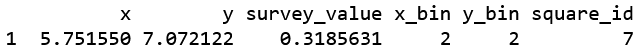
\includegraphics{Templates/Screenshot 2023-02-21 at 17-02-20 RStudio Server.png}
\caption{unchanged image}
\end{figure}

Chaque carré ayant un identifiant, nous pouvons lui affecter une donnée
de contexte.

\begin{Shaded}
\begin{Highlighting}[]
\CommentTok{\#Ajout de la colonne correspondant à la valeur de chaque carré}
\NormalTok{df}\SpecialCharTok{$}\NormalTok{square\_value }\OtherTok{\textless{}{-}}\NormalTok{ square\_values[df}\SpecialCharTok{$}\NormalTok{square\_id]}
\end{Highlighting}
\end{Shaded}

La grille est donc bien modélisée selon le tableau suivant :

\begin{Shaded}
\begin{Highlighting}[]
\FunctionTok{head}\NormalTok{(df)}
\end{Highlighting}
\end{Shaded}

\begin{verbatim}
##     x   y survey_value x_bin y_bin square_id square_value
## 1 0.5 0.5    0.9647704     1     1         1    0.9295728
## 2 1.5 1.5    0.9817934     1     1         1    0.9295728
## 3 2.5 2.5    0.3526031     2     2        11    0.7822874
## 4 3.5 3.5    0.9364447     2     2        11    0.7822874
## 5 4.5 4.5    0.1033376     3     3        21    0.1745220
## 6 5.5 5.5    0.4778902     3     3        21    0.1745220
\end{verbatim}

Voici à quoi pourrait typiquement ressembler les données sur lesquelles
on souhaiterait appliquer une agrégation géographique avec contrainte de
contiguïté.

\hypertarget{repruxe9sentation-graphique-de-notre-grille}{%
\section{Représentation graphique de notre
grille}\label{repruxe9sentation-graphique-de-notre-grille}}

L'image est considérée comme trop grande à partir d'une grille de
dimension 10x10. La grille sera tout de même modélisée mais il faudra
adapter sa RAM si l'utilisateur tient à afficher la grille complète des
individus simulés.

\begin{verbatim}
## Warning: The `size` argument of `element_line()` is deprecated as of ggplot2 3.4.0.
## i Please use the `linewidth` argument instead.
\end{verbatim}

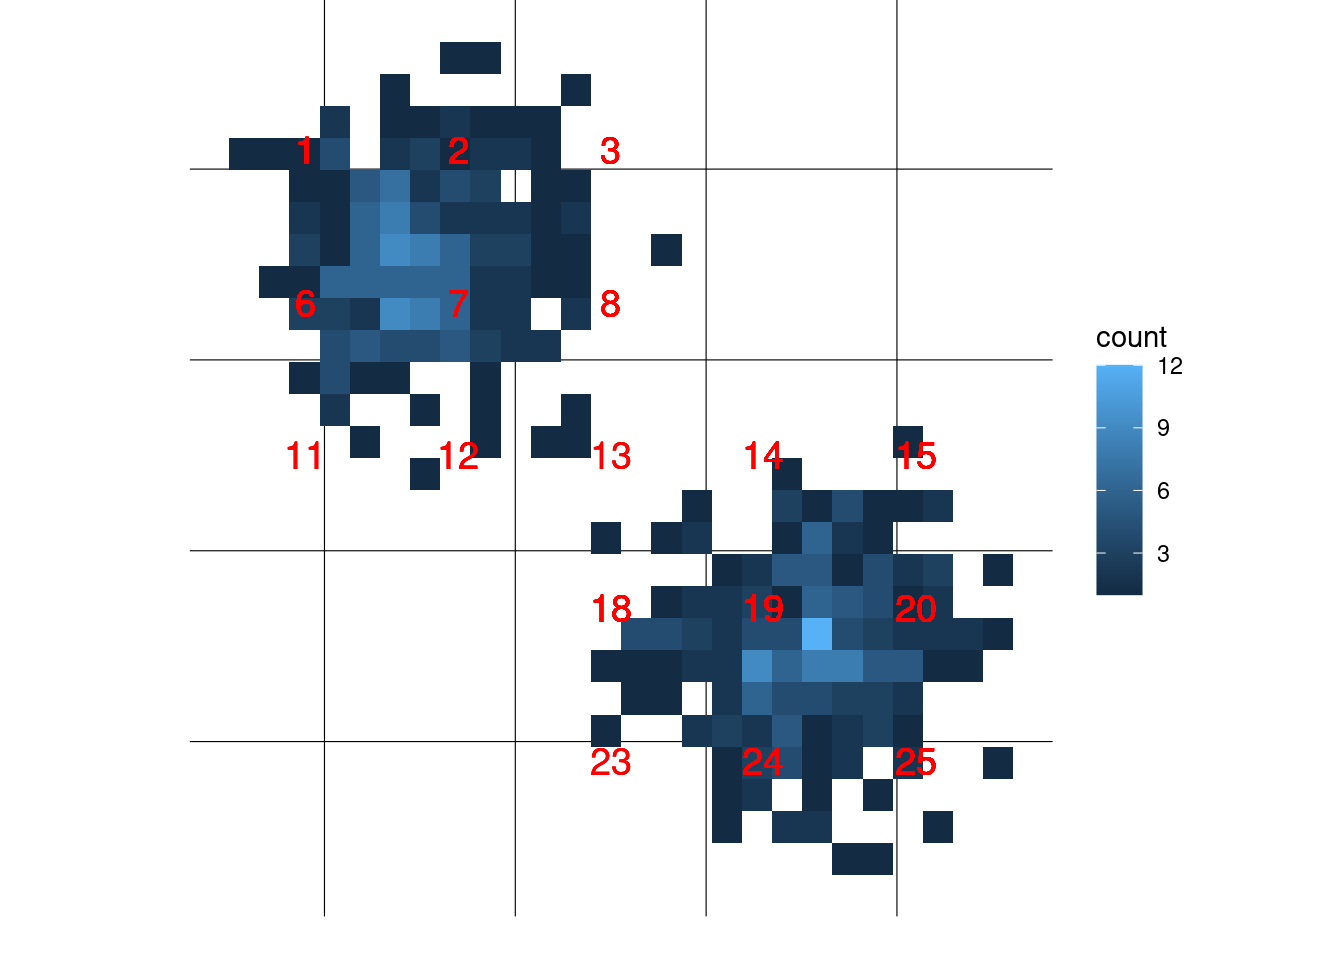
\includegraphics{Markdown_Projet_Methodo_files/figure-latex/unnamed-chunk-11-1.pdf}

\hypertarget{mise-en-forme-du-tableau-traitement-des-donnuxe9es-simuluxe9es-pour-uxeatre-fournies-en-entruxe9e-uxe0-notre-algorithme-dagruxe9gation}{%
\section{Mise en forme du tableau : Traitement des données simulées pour
être fournies en entrée à notre algorithme
d'agrégation}\label{mise-en-forme-du-tableau-traitement-des-donnuxe9es-simuluxe9es-pour-uxeatre-fournies-en-entruxe9e-uxe0-notre-algorithme-dagruxe9gation}}

Nous renommons et filtrons les variables pertinentes pour une meilleure
compréhension dans le contexte du problème. Nous n'avons besoin que des
données des contexte et les identifiants des communes. Il nous reste le
nombre de répondants à l'enquête par commune.

\begin{Shaded}
\begin{Highlighting}[]
\CommentTok{\#Restitution du tableau final qui va être utilisé}
\NormalTok{df}\SpecialCharTok{$}\NormalTok{coords }\OtherTok{\textless{}{-}} \FunctionTok{paste}\NormalTok{(df}\SpecialCharTok{$}\NormalTok{x, df}\SpecialCharTok{$}\NormalTok{y, }\AttributeTok{sep =} \StringTok{","}\NormalTok{)}
\CommentTok{\#Filtrer les données et renommer les colonnes}
\NormalTok{donnees }\OtherTok{\textless{}{-}}\NormalTok{ dplyr}\SpecialCharTok{::}\FunctionTok{select}\NormalTok{(df,square\_value,square\_id)}
\FunctionTok{colnames}\NormalTok{(donnees) }\OtherTok{\textless{}{-}} \FunctionTok{c}\NormalTok{(}\StringTok{"donnee\_contexte\_commune"}\NormalTok{, }\StringTok{"ID"}\NormalTok{)}
\end{Highlighting}
\end{Shaded}

\hypertarget{moduxe9lisation-des-enquuxeatuxe9s}{%
\subsection{Modélisation des
enquêtés}\label{moduxe9lisation-des-enquuxeatuxe9s}}

\hypertarget{indicatrice-de-ruxe9ponse-uxe0-lenquuxeate}{%
\subsubsection{Indicatrice de réponse à
l'enquête}\label{indicatrice-de-ruxe9ponse-uxe0-lenquuxeate}}

Nous simulons le fait que des individus ont répondu à une enquête dans
chaque carré les individus qui ont répondu à une enquête en effectuant
un tirage de Bernoulli selon la variable correspondant aux données de
contexte. Cela permet de modéliser le fait que plus la variable
d'intérêt est grande plus il y a de chances d'avoir de répondants.

\textbf{Première option} : Nous tirons simplement des individus au
hasard sur tout le territoire. \textbf{Deuxième option} : Nous
effectuons un échantillonage à deux degrés en ayant pour unité primaire
les communes et comme unité secondaire les individus.

Nous privilégions la seconde option qui est davantage dans l'esprit du
papier \emph{Un algorithme de regroupement d'unités statistiques selon
certains critères de similitude} écrit par Michel Isnard et Marc
Christine. De plus, il y a un gain potentiel de variance par rapport à
un échantillonnage directement sur les individus du territoire
métropolitain français, en particulier si la variable d'intérêt varie
considérablement entre les communes. Nous nous assurons alors que
l'échantillon obtenu est représentatif des différentes strates de la
population étudiée (les communes dans ce cas), ce qui peut permettre de
réduire la variance de l'estimateur de la moyenne ou de la proportion.

Autre avantage du tirage à deux degrés: améliorer l'estimation de la
taille des unités primaires, dans ce cas les communes (ou carrés). Nous
verrons en quoi cela peut-être intéressant lors de l'implémentation de
la distance de similarité.

Nous créons donc une variable binaire ``inclusion\_enquete'' qui
renseigne si un individu est sélectionné dans l'enquête.

\hypertarget{impluxe9mentation-de-la-premiuxe8re-option-de-tirage-non-exuxe9cutuxe9e-evalfalse}{%
\paragraph{Implémentation de la première option de tirage (non exécutée:
eval=FALSE)}\label{impluxe9mentation-de-la-premiuxe8re-option-de-tirage-non-exuxe9cutuxe9e-evalfalse}}

\begin{Shaded}
\begin{Highlighting}[]
\CommentTok{\# Effectuer le tirage de Bernoulli selon les données de contexte pour chaque carré}
\NormalTok{donnees}\SpecialCharTok{$}\NormalTok{inclusion\_enquete }\OtherTok{\textless{}{-}} \FunctionTok{rbinom}\NormalTok{(}\FunctionTok{nrow}\NormalTok{(donnees), }\DecValTok{1}\NormalTok{, donnees}\SpecialCharTok{$}\NormalTok{donnee\_contexte\_commune)}

\CommentTok{\# Calculer la probabilité d\textquotesingle{}inclusion pour chaque individu}
\NormalTok{prob\_inclusion }\OtherTok{\textless{}{-}} \FunctionTok{ave}\NormalTok{(donnees}\SpecialCharTok{$}\NormalTok{inclusion\_enquete, donnees}\SpecialCharTok{$}\NormalTok{ID, }\AttributeTok{FUN =} \ControlFlowTok{function}\NormalTok{(x) }\FunctionTok{sum}\NormalTok{(x)}\SpecialCharTok{/}\FunctionTok{length}\NormalTok{(x))}
\NormalTok{donnees}\SpecialCharTok{$}\NormalTok{proba\_inclusion\_enquete }\OtherTok{\textless{}{-}}\NormalTok{ prob\_inclusion[donnees}\SpecialCharTok{$}\NormalTok{ID]}

\CommentTok{\# Afficher les carrés inclus dans l\textquotesingle{}échantillon}
\NormalTok{echantillon }\OtherTok{\textless{}{-}}\NormalTok{ donnees[donnees}\SpecialCharTok{$}\NormalTok{inclusion\_enquete }\SpecialCharTok{==} \DecValTok{1}\NormalTok{, ]}
\FunctionTok{cat}\NormalTok{(}\StringTok{"Le nombre d\textquotesingle{}individus enquêté est de"}\NormalTok{, }\FunctionTok{dim}\NormalTok{(echantillon)[}\DecValTok{1}\NormalTok{])}
\end{Highlighting}
\end{Shaded}

\begin{verbatim}
## Le nombre d'individus enquêté est de 4416
\end{verbatim}

\#\#\#\#Implémentation de la seconde option de tirage

\begin{Shaded}
\begin{Highlighting}[]
\CommentTok{\# Nombre d\textquotesingle{}unités primaires à tirer, ici les communes}
\NormalTok{n\_up\_sample }\OtherTok{\textless{}{-}} \DecValTok{10}

\CommentTok{\# Tirage des unités primaires au hasard}
\FunctionTok{set.seed}\NormalTok{(}\DecValTok{123}\NormalTok{) }\CommentTok{\# pour reproduire les résultats}
\NormalTok{up\_sample }\OtherTok{\textless{}{-}} \FunctionTok{sample}\NormalTok{(}\FunctionTok{unique}\NormalTok{(donnees}\SpecialCharTok{$}\NormalTok{ID), n\_up\_sample)}

\CommentTok{\# Sous{-}échantillonnage des unités secondaires pour chaque unité primaire sélectionnée}
\NormalTok{donnees\_subsampled }\OtherTok{\textless{}{-}}\NormalTok{ donnees }\SpecialCharTok{\%\textgreater{}\%}
  \FunctionTok{filter}\NormalTok{(ID }\SpecialCharTok{\%in\%}\NormalTok{ up\_sample) }\SpecialCharTok{\%\textgreater{}\%}
  \FunctionTok{group\_by}\NormalTok{(ID) }\SpecialCharTok{\%\textgreater{}\%}
  \FunctionTok{sample\_n}\NormalTok{(}\FunctionTok{ceiling}\NormalTok{(}\FloatTok{0.5} \SpecialCharTok{*} \FunctionTok{n}\NormalTok{()))}

\CommentTok{\# Calcul des probabilités d\textquotesingle{}inclusion pour chaque unité secondaire}
\NormalTok{donnees\_subsampled}\SpecialCharTok{$}\NormalTok{proba\_inclusion }\OtherTok{\textless{}{-}}\NormalTok{ donnees\_subsampled}\SpecialCharTok{$}\NormalTok{donnee\_contexte\_commune}
\end{Highlighting}
\end{Shaded}

\hypertarget{duxe9finition-des-zones-dabsence-denquuxeatuxe9}{%
\subsubsection{Définition des zones d'absence
d'enquêté}\label{duxe9finition-des-zones-dabsence-denquuxeatuxe9}}

Nous définissons des zones très vides au niveau de l'enquête pour
observer comment ces zones particulières seront agrégées. L'intérêt est
d'observer s'il est possible d'obtenir un gros agrégat sans répondants.
Que faire si cela arrive ? Il semble que cela n'arrive pas pour notre
algorithme.

Nous définissons la zone manuellement pour être sûr d'avoir un bloc
d'absence de répondants mais il est possible d'automatiser en prenant un
certain nombre de communes voisines ne se trouvant pas en métropole ou
dans d'autres zones souhaitées. Si c'est ce que l'on souhaite,
l'utilisateur doit créer une variable d'appartenance à une métropole et
reprendre le principe de notre ligne de code ci-dessous. On souhaite
qu'en donnant une proportion

\begin{Shaded}
\begin{Highlighting}[]
\CommentTok{\# Remplacer la variable inclusion\_enquete à 0 pour certains}
\NormalTok{donnees}\SpecialCharTok{$}\NormalTok{inclusion\_enquete }\OtherTok{\textless{}{-}} \FunctionTok{ifelse}\NormalTok{(donnees}\SpecialCharTok{$}\NormalTok{ID }\SpecialCharTok{\%in\%} \FunctionTok{c}\NormalTok{(}\DecValTok{43}\NormalTok{,}\DecValTok{44}\NormalTok{,}\DecValTok{45}\NormalTok{,}\DecValTok{52}\NormalTok{,}\DecValTok{53}\NormalTok{,}\DecValTok{54}\NormalTok{,}\DecValTok{61}\NormalTok{,}\DecValTok{62}\NormalTok{,}\DecValTok{63}\NormalTok{,}\DecValTok{77}\NormalTok{,}\DecValTok{78}\NormalTok{,}\DecValTok{79}\NormalTok{), }\DecValTok{0}\NormalTok{, donnees}\SpecialCharTok{$}\NormalTok{inclusion\_enquete)}
\end{Highlighting}
\end{Shaded}

\hypertarget{visualisation-des-enquuxeatuxe9s-selectionnuxe9s-sur-le-territoire}{%
\paragraph{Visualisation des enquêtés selectionnés sur le
territoire}\label{visualisation-des-enquuxeatuxe9s-selectionnuxe9s-sur-le-territoire}}

\includegraphics{Markdown_Projet_Methodo_files/figure-latex/unnamed-chunk-16-1.pdf}

\hypertarget{agruxe9gation-uxe0-luxe9chelle-des-communes}{%
\subsubsection{Agrégation à l'échelle des
communes}\label{agruxe9gation-uxe0-luxe9chelle-des-communes}}

Pour avoir le nombre de répondants à l'enquête dans chaque commune, nous
agrégons ensuite les données individuelles à l'échelle des communes.

Les données sont fin prêtes pour l'agrégation.

\begin{Shaded}
\begin{Highlighting}[]
\FunctionTok{head}\NormalTok{(donnees\_agg)}
\end{Highlighting}
\end{Shaded}

\begin{verbatim}
## # A tibble: 6 x 5
## # Groups:   ID [6]
##      ID donnee_contexte_commune nb_repondants_commune taille_commune somme_pro~1
##   <dbl>                   <dbl>                 <dbl>          <dbl>       <dbl>
## 1     1                   0.930                    22             22       22   
## 2     2                   0.172                     5             45       45   
## 3     3                   0.807                    34             37       29.3 
## 4     4                   0.284                     7             23       18.2 
## 5     5                   0.317                    10             34        6.36
## 6     6                   0.141                    16            113       21.1 
## # ... with abbreviated variable name 1: somme_proba_inclusion_enquete
\end{verbatim}

\hypertarget{observation-du-lien-entre-donnuxe9es-de-contexte-et-nombre-de-ruxe9pondants}{%
\subsection{Observation du lien entre données de contexte et nombre de
répondants}\label{observation-du-lien-entre-donnuxe9es-de-contexte-et-nombre-de-ruxe9pondants}}

Nous avons une structure des données de contexte qui affecte
positivement avec le nombre de répondants. Observe t-on une corrélation
entre les données de contexte et le nombre de répondants ?

\begin{Shaded}
\begin{Highlighting}[]
\FunctionTok{plot}\NormalTok{(donnees\_agg}\SpecialCharTok{$}\NormalTok{nb\_repondants\_commune,donnees\_agg}\SpecialCharTok{$}\NormalTok{donnee\_contexte\_commune)}
\end{Highlighting}
\end{Shaded}

\includegraphics{Markdown_Projet_Methodo_files/figure-latex/unnamed-chunk-19-1.pdf}

\hypertarget{codification-de-la-structure-de-voisinage}{%
\section{Codification de la structure de
voisinage}\label{codification-de-la-structure-de-voisinage}}

Il est important de définir la notion de voisinage car elle diffère
selon le type que l'on a choisie. Les deux types de voisinages les plus
usuels sont la contiguïté ``QUEEN'' et ``ROOK'', analogue au possibilité
de déplacement des pièces correspondantes aux jeux d'échecs.

\begin{figure}
\centering
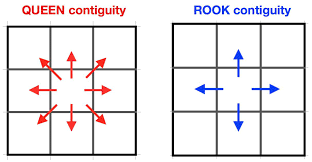
\includegraphics{Templates/contiguite.png}
\caption{unchanged image}
\end{figure}

En pratique, il faut renseigner les voisins à la main. Dans le cadre
d'une grille de commune, il est possible d'écrire un algorithme pour
définir une structure de voisinage en raisonnant sur les identifiants
des communes. En utilisant des considérations arithmétiques et en
traitant les cas particuliers (carrés sur les bords gauche et droite),
il est possible d'écrire cela pour notre grille 25x25.

\hypertarget{cruxe9ation-de-la-matrice-de-contiguuxeftuxe9}{%
\subsection{Création de la matrice de
contiguïté}\label{cruxe9ation-de-la-matrice-de-contiguuxeftuxe9}}

Nous créons deux fonctions codant les deux différents types de
voisinage. Pour la suite, nous appliquerons la contiguité ROOK i.e il ne
suffit pas qu'elles partagent un point de frontière commune pour que
deux communes soient voisines.

Choisir le type de contiguïté revient de manière équivalente à choisir
une certaine distance à appliquer entre deux indices de carré dans une
grille (ou un damier) et de ne garder que les voisins directs i.e qui
n'ont qu'une distance de 1 avec le carré considéré.

Exemple: avec la distance de Tchebychev, les voisins directs du roi ont
une distance de 1 et on ne retient qu ceux-là. La distance de Manhattan
donnent les mêmes résultats mais sans les diagonales. Nous implémentons
donc ces distances pour créer notre matrice de contiguïté.

\begin{figure}
\centering
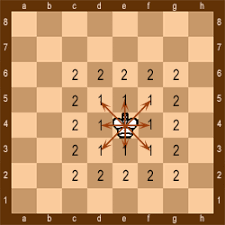
\includegraphics{Templates/chebychev.png}
\caption{unchanged image}
\end{figure}

Les fonctions implémentées suivantes s'inspirent des distances de
Manhattan et de Chebychev entre deux carrés du damier dont les indices
sont i et j, sans tenir compte de leur position réelle dans l'espace.

Si l'on souhaite expérimenter d'autres distances plus exotiques, il est
possible de les implémenter ci-dessous et de les rajouter dans le code
qui suit.

\begin{Shaded}
\begin{Highlighting}[]
\NormalTok{distance\_tchebychev\_indices}\OtherTok{=}\ControlFlowTok{function}\NormalTok{(i,j)\{}\FunctionTok{return}\NormalTok{(}\FunctionTok{max}\NormalTok{(}\FunctionTok{abs}\NormalTok{((j}\DecValTok{{-}1}\NormalTok{) }\SpecialCharTok{\%/\%}\NormalTok{ n }\SpecialCharTok{{-}}\NormalTok{ (i}\DecValTok{{-}1}\NormalTok{) }\SpecialCharTok{\%/\%}\NormalTok{ n), }\FunctionTok{abs}\NormalTok{((j}\DecValTok{{-}1}\NormalTok{) }\SpecialCharTok{\%\%}\NormalTok{ n }\SpecialCharTok{{-}}\NormalTok{ (i}\DecValTok{{-}1}\NormalTok{) }\SpecialCharTok{\%\%}\NormalTok{ n))) \}}
\NormalTok{distance\_manhattan\_indices}\OtherTok{=}\ControlFlowTok{function}\NormalTok{(i,j)\{}\FunctionTok{return}\NormalTok{(}\FunctionTok{abs}\NormalTok{((j}\DecValTok{{-}1}\NormalTok{) }\SpecialCharTok{\%/\%}\NormalTok{ n }\SpecialCharTok{{-}}\NormalTok{ (i}\DecValTok{{-}1}\NormalTok{) }\SpecialCharTok{\%/\%}\NormalTok{ n) }\SpecialCharTok{+} \FunctionTok{abs}\NormalTok{((j}\DecValTok{{-}1}\NormalTok{) }\SpecialCharTok{\%\%}\NormalTok{ n }\SpecialCharTok{{-}}\NormalTok{ (i}\DecValTok{{-}1}\NormalTok{) }\SpecialCharTok{\%\%}\NormalTok{ n)) \}}
\end{Highlighting}
\end{Shaded}

\begin{Shaded}
\begin{Highlighting}[]
\NormalTok{create\_contig\_matrix }\OtherTok{=} \ControlFlowTok{function}\NormalTok{(n, }\AttributeTok{type=}\StringTok{"Rook"}\NormalTok{)\{}
\NormalTok{a }\OtherTok{\textless{}{-}}\NormalTok{ b }\OtherTok{\textless{}{-}} \FunctionTok{c}\NormalTok{()}
\ControlFlowTok{for}\NormalTok{ (i }\ControlFlowTok{in} \DecValTok{1}\SpecialCharTok{:}\NormalTok{(n}\SpecialCharTok{\^{}}\DecValTok{2}\NormalTok{)) \{}
  \ControlFlowTok{for}\NormalTok{ (j }\ControlFlowTok{in} \DecValTok{1}\SpecialCharTok{:}\NormalTok{(n}\SpecialCharTok{\^{}}\DecValTok{2}\NormalTok{)) \{}
    \FunctionTok{ifelse}\NormalTok{(type}\SpecialCharTok{==}\StringTok{"Rook"}\NormalTok{,diff }\OtherTok{\textless{}{-}} \FunctionTok{distance\_manhattan\_indices}\NormalTok{(i,j),}\FunctionTok{ifelse}\NormalTok{(type}\SpecialCharTok{==}\StringTok{"Queen"}\NormalTok{,diff }\OtherTok{\textless{}{-}} \FunctionTok{distance\_tchebychev\_indices}\NormalTok{(i,j),}\StringTok{"Précisez un type de contiguïté existant: Rook ou Queen"}\NormalTok{) )}
    \CommentTok{\# la condition diff \textgreater{} 1 permet de filtrer les paires de carrés qui ne sont pas des voisins directs}
    \CommentTok{\# la condition i \textgreater{}= j permet d\textquotesingle{}éviter les doublo}
    \ControlFlowTok{if}\NormalTok{ (diff }\SpecialCharTok{\textgreater{}} \DecValTok{1} \SpecialCharTok{||}\NormalTok{ i }\SpecialCharTok{\textgreater{}=}\NormalTok{ j) \{}
      \ControlFlowTok{next}
\NormalTok{    \} }\ControlFlowTok{else}\NormalTok{ \{}
\NormalTok{      a }\OtherTok{\textless{}{-}} \FunctionTok{c}\NormalTok{(a, i)}
\NormalTok{      b }\OtherTok{\textless{}{-}} \FunctionTok{c}\NormalTok{(b, j)}
\NormalTok{    \}}
\NormalTok{  \}}
\NormalTok{\}}
\NormalTok{voisin }\OtherTok{\textless{}{-}} \FunctionTok{cbind}\NormalTok{(a, b)}
\FunctionTok{colnames}\NormalTok{(voisin) }\OtherTok{\textless{}{-}} \FunctionTok{c}\NormalTok{(}\StringTok{"id1"}\NormalTok{,}\StringTok{"id2"}\NormalTok{)}
\NormalTok{voisin }\OtherTok{\textless{}{-}} \FunctionTok{data.frame}\NormalTok{(voisin)}
\CommentTok{\#conversion des colonnes en chaine de caracteres}
\NormalTok{voisin}\SpecialCharTok{$}\NormalTok{id1 }\OtherTok{\textless{}{-}} \FunctionTok{as.character}\NormalTok{(voisin}\SpecialCharTok{$}\NormalTok{id1)}
\NormalTok{voisin}\SpecialCharTok{$}\NormalTok{id2 }\OtherTok{\textless{}{-}} \FunctionTok{as.character}\NormalTok{(voisin}\SpecialCharTok{$}\NormalTok{id2)}
\CommentTok{\#conversion en tibble pour les fonctions d\textquotesingle{}aggrégation}
\NormalTok{contig\_matrix }\OtherTok{\textless{}{-}} \FunctionTok{as.matrix}\NormalTok{(voisin)}
\FunctionTok{return}\NormalTok{(contig\_matrix)}
\NormalTok{\}}
\end{Highlighting}
\end{Shaded}

Nous pouvons enfin créer notre matrice de contiguïté. Nous renseignons
en argument de la fonction le nombre de carrés que l'on a sur une rangée
(ligne ou colonne)

\begin{Shaded}
\begin{Highlighting}[]
\NormalTok{contig\_matrix }\OtherTok{\textless{}{-}} \FunctionTok{create\_contig\_matrix}\NormalTok{(nb\_cols\_squares)}
\end{Highlighting}
\end{Shaded}

Si l'on préfère la contiguité Queen, on peut rajouter l'argument
``Queen'' comme ci-dessous :

\begin{Shaded}
\begin{Highlighting}[]
\FunctionTok{create\_contig\_matrix}\NormalTok{(}\FunctionTok{sqrt}\NormalTok{(nb\_cols\_squares),}\StringTok{"Queen"}\NormalTok{)}
\end{Highlighting}
\end{Shaded}

\hypertarget{mise-en-place-de-lagruxe9gation}{%
\section{Mise en place de
l'agrégation}\label{mise-en-place-de-lagruxe9gation}}

\hypertarget{clustering-avec-contraintes-de-contiguuxeftuxe9-et-crituxe8re-darruxeat-sur-les-ruxe9pondants}{%
\subsection{Clustering avec contraintes de contiguïté et critère d'arrêt
sur les
répondants}\label{clustering-avec-contraintes-de-contiguuxeftuxe9-et-crituxe8re-darruxeat-sur-les-ruxe9pondants}}

Nous définissons différentes fonctions utilitaires pour la gestion des
contraintes.

\hypertarget{fonction-de-contiguuxeftuxe9}{%
\subsubsection{Fonction de
contiguïté}\label{fonction-de-contiguuxeftuxe9}}

Nous créons une fonction qui vérifie si 2 agrégats i et j sont
géographiquement voisins selon la matrice de contiguïté que nous avons
définie. Chaque agrégat contient plusieurs communes. La convention que
nous avons choisie pour dire que 2 agrégats sont voisins est de regarder
si au moins une commune d'un agrégat est voisine au minimum avec une
commune de l'autre agrégat.

\begin{Shaded}
\begin{Highlighting}[]
\NormalTok{groupes\_voisins }\OtherTok{\textless{}{-}} \ControlFlowTok{function}\NormalTok{(groups,i,j)\{ }\CommentTok{\#fonction qui évalue si les agrégats i et j sont voisins}
\NormalTok{  res}\OtherTok{=}\NormalTok{F}
  \ControlFlowTok{for}\NormalTok{ (k }\ControlFlowTok{in} \DecValTok{1}\SpecialCharTok{:}\FunctionTok{length}\NormalTok{(contig\_matrix[,}\DecValTok{1}\NormalTok{]))\{}
    \ControlFlowTok{for}\NormalTok{ (x }\ControlFlowTok{in}\NormalTok{ groups[[i]])\{}
      \ControlFlowTok{for}\NormalTok{ (y }\ControlFlowTok{in}\NormalTok{ groups[[j]])\{}
        \ControlFlowTok{if}\NormalTok{((contig\_matrix[k,}\StringTok{"id1"}\NormalTok{]}\SpecialCharTok{==}\NormalTok{x }\SpecialCharTok{\&\&}\NormalTok{ contig\_matrix[k,}\StringTok{"id2"}\NormalTok{]}\SpecialCharTok{==}\NormalTok{y)}\SpecialCharTok{|}\NormalTok{(contig\_matrix[k,}\StringTok{"id1"}\NormalTok{]}\SpecialCharTok{==}\NormalTok{y }\SpecialCharTok{\&\&}\NormalTok{ contig\_matrix[k,}\StringTok{"id2"}\NormalTok{]}\SpecialCharTok{==}\NormalTok{x))\{}
\NormalTok{          res}\OtherTok{=}\NormalTok{T}
\NormalTok{        \}}
\NormalTok{      \}}
\NormalTok{    \}}
\NormalTok{  \}}
  \FunctionTok{return}\NormalTok{(res)}
\NormalTok{\}}
\end{Highlighting}
\end{Shaded}

\hypertarget{plusieurs-fonctions-de-distance-possibles-selon-les-besoins}{%
\subsubsection{Plusieurs fonctions de distance possibles selon les
besoins}\label{plusieurs-fonctions-de-distance-possibles-selon-les-besoins}}

Dans le cas où les agrégats ne contiennent qu'une commune, nous voulons
choisir la fonction de distance appropriée. Pour modéliser nos données
de contexte, nous avons choisi une proportion qui pourrait par exemple
représenter le taux de tabagisme dans la commune mais ce n'est pas le
seul type de variable possible. Nous laissons dons le choix à
l'utilisateur de choisir la distance qui correspond au mieux aux données
de contexte. Il a la possibilité d'implémenter d'autres distances entre
les agrégats

\hypertarget{quelques-distances-basiques-si-nous-navons-pas-de-contraintes-particuliuxe8res.}{%
\paragraph{Quelques distances basiques si nous n'avons pas de
contraintes
particulières.}\label{quelques-distances-basiques-si-nous-navons-pas-de-contraintes-particuliuxe8res.}}

Nous avons quelques distances selon si les données de contexte sont
qualitatives ou quantitatives. Pour les variables continues: possibilité
d'utiliser la distance de Mahalanobis ou de Manhattan Pour les variables
catégorielles: possibilité d'utiliser la distance de Jaccard ou de
Hamming

\begin{Shaded}
\begin{Highlighting}[]
\CommentTok{\# Pour des variables continues}
\CommentTok{\#Pour la distance de Mahalanobis, il faut spécifier la matrice de covariance comme argument.}
\NormalTok{distance\_mahalanobis }\OtherTok{\textless{}{-}} \ControlFlowTok{function}\NormalTok{(mean1, mean2, cov) \{}
  \FunctionTok{sqrt}\NormalTok{((mean1 }\SpecialCharTok{{-}}\NormalTok{ mean2) }\SpecialCharTok{\%*\%} \FunctionTok{solve}\NormalTok{(cov) }\SpecialCharTok{\%*\%} \FunctionTok{t}\NormalTok{(mean1 }\SpecialCharTok{{-}}\NormalTok{ mean2))}
\NormalTok{\}}
\NormalTok{distance\_manhattan }\OtherTok{\textless{}{-}} \ControlFlowTok{function}\NormalTok{(mean1, mean2) \{}
  \FunctionTok{sum}\NormalTok{(}\FunctionTok{abs}\NormalTok{(mean1 }\SpecialCharTok{{-}}\NormalTok{ mean2))}
\NormalTok{\}}
\CommentTok{\# Pour des variables catégorielles}
\NormalTok{distance\_Jaccard }\OtherTok{\textless{}{-}} \ControlFlowTok{function}\NormalTok{(data\_group1, data\_group2) \{}
  \CommentTok{\# Nombre d\textquotesingle{}éléments dans les deux groupes combinés}
\NormalTok{  n }\OtherTok{\textless{}{-}} \FunctionTok{length}\NormalTok{(}\FunctionTok{union}\NormalTok{(data\_group1, data\_group2))}
  \CommentTok{\# Nombre d\textquotesingle{}éléments communs aux deux groupes}
\NormalTok{  n\_common }\OtherTok{\textless{}{-}} \FunctionTok{length}\NormalTok{(}\FunctionTok{intersect}\NormalTok{(data\_group1, data\_group2))}
  \CommentTok{\# Calcul de la distance de Jaccard}
\NormalTok{  dist\_jaccard }\OtherTok{\textless{}{-}} \DecValTok{1} \SpecialCharTok{{-}}\NormalTok{ n\_common }\SpecialCharTok{/}\NormalTok{ n}
  \FunctionTok{return}\NormalTok{(dist\_jaccard)}
\NormalTok{\}}
\CommentTok{\#par vote majoritaire}
\NormalTok{distance\_Hamming }\OtherTok{\textless{}{-}} \ControlFlowTok{function}\NormalTok{(data\_group1, data\_group2)\{}
  \CommentTok{\# Calcul de la distance de Hamming entre deux groupes}
\NormalTok{  dist\_hamming }\OtherTok{\textless{}{-}} \FunctionTok{sum}\NormalTok{(data\_group1 }\SpecialCharTok{!=}\NormalTok{ data\_group2)}
  \FunctionTok{return}\NormalTok{(dist\_hamming)}
\NormalTok{\}}
\end{Highlighting}
\end{Shaded}

\hypertarget{distance-de-ward.d2-pour-avoir-les-agruxe9gats-les-plus-homoguxe8nes-possibles}{%
\paragraph{Distance de Ward.D2 : pour avoir les agrégats les plus
homogènes
possibles}\label{distance-de-ward.d2-pour-avoir-les-agruxe9gats-les-plus-homoguxe8nes-possibles}}

Nous souhaitons regrouper les communes qui se ressemblent le plus en
terme de données de contexte. Les communes doivent donc être les plus
homogènes possibles au sein d'un agrégat et les agrégats doivent être
les plus différents possibles. En conséquence, la fonction est donc
construite sur les données de contexte associées à chaque commune.

Pour cela, nous choisissons une mesure de similarité très performante
pour répondre à notre besoin, et classiquement utilisé pour le
clustering hiérarchique (notamment populaire avec le langage R). Il
s'agit de la distance de Ward.D2 dont l'implémentation est détaillée
dans ``Ward's Hierarchical Clustering Method:Clustering Criterion and
Agglomerative Algorithm'', Pierre Legendre, Fionn Murtagh. L'écart de
Ward est une méthode de liaison qui cherche à minimiser la somme des
carrés des différences entre chaque individu et la moyenne de son
groupe, tout en maximisant la séparation entre les groupes. Cette
méthode prend en compte les distances entre les individus, mais pas la
distance absolue.

Pour expliquer brièvement le principe, elle mesure la variance totale
des deux agrégats à fusionner. Elle est calculée en comparant la somme
des carrés des distances de chaque point à son centre de gravité dans
chaque agrégat. Cette distance mesure ainsi la différence entre la somme
des carrés des distances de chaque objet dans le même agrégat et la
somme des carrés des distances de chaque objet dans des agrégats
différents.

\begin{Shaded}
\begin{Highlighting}[]
\NormalTok{distance\_Ward.D2 }\OtherTok{\textless{}{-}} \ControlFlowTok{function}\NormalTok{(data\_group1,data\_group2,mean1,mean2)\{}
  \CommentTok{\# Calcul de la somme des carrés des écarts à la moyenne pour chaque groupe}
\NormalTok{  ssd1 }\OtherTok{\textless{}{-}} \FunctionTok{sum}\NormalTok{((data\_group1 }\SpecialCharTok{{-}}\NormalTok{ mean1) }\SpecialCharTok{\^{}} \DecValTok{2}\NormalTok{)}
\NormalTok{  ssd2 }\OtherTok{\textless{}{-}} \FunctionTok{sum}\NormalTok{((data\_group2 }\SpecialCharTok{{-}}\NormalTok{ mean2) }\SpecialCharTok{\^{}} \DecValTok{2}\NormalTok{)}
  \CommentTok{\# Calcul de la somme des carrés des écarts à la moyenne pour tous les points}
\NormalTok{  ssd\_all }\OtherTok{\textless{}{-}} \FunctionTok{sum}\NormalTok{((}\FunctionTok{c}\NormalTok{(data\_group1,data\_group2) }\SpecialCharTok{{-}}\NormalTok{ mean\_all) }\SpecialCharTok{\^{}} \DecValTok{2}\NormalTok{)}
  \CommentTok{\# Calcul de la distance entre deux groupes pour la méthode ward.d2}
\NormalTok{  dist\_between\_groups }\OtherTok{\textless{}{-}}\NormalTok{ ssd\_all }\SpecialCharTok{{-}}\NormalTok{ (ssd1 }\SpecialCharTok{+}\NormalTok{ ssd2)}
  \FunctionTok{return}\NormalTok{(}\FunctionTok{sqrt}\NormalTok{(dist\_between\_groups }\SpecialCharTok{/}\NormalTok{ (}\FunctionTok{length}\NormalTok{(data\_group1)}\SpecialCharTok{+}\FunctionTok{length}\NormalTok{(data\_group2))))}
\NormalTok{\}}
\end{Highlighting}
\end{Shaded}

\hypertarget{distance-ponduxe9ruxe9e}{%
\paragraph{Distance pondérée}\label{distance-ponduxe9ruxe9e}}

La mesure de similarité précédente prend en compte des considérations
purement statistiques mais comme nous nous trouvons dans le cadre d'un
thème précis qui est la classification \textbf{géographique}, il est
possible voire davantage cohérent de tirer profit d'une pondération des
communes.

Tout comme, il est proposé dans le code proposé par M. Hisnard,
``l'utilisateur est évidemment libre de choisir toute autre distance. Il
convient de remarquer que le choix de la distance peut influer sur la
taille des classe créées, par-là sur le nombre de voisins à chaque
itération et donc sur la durée du programme.''

Plutôt que la distance de Ward.D2 classique, il peut être intéressant de
regarder celle entre deux unités dans un ensemble de données, en prenant
en compte une variable pondérée nommée ``Poids''. ( explication d'ajout
du terme P1*P2/(P1+P2)). En effet, certaines méthodes de regroupement,
comme l'écart de Ward, peuvent être plus sensibles aux différences de
taille entre les clusters. Dans ces cas, il peut être utile de
normaliser la distance entre les individus avant de calculer la distance
entre les clusters pour éviter que les différences de taille ne dominent
le processus de regroupement.

Dans notre cas, nous allons simplement adapter le code en calculant une
moyenne pondérée des individus à la place d'une moyenne classique.

Nous pouvons donc calculer une fonction de distance euclidienne pondérée
comme ci-dessus comme recherché par Hisnard.

\begin{Shaded}
\begin{Highlighting}[]
\NormalTok{distance\_euclidienne\_ponderee }\OtherTok{\textless{}{-}} \ControlFlowTok{function}\NormalTok{(data\_group1,data\_group2,mean1\_ponderee, mean2\_ponderee,w1,w2) \{}
  \FunctionTok{sqrt}\NormalTok{(}\FunctionTok{sum}\NormalTok{((mean1\_ponderee }\SpecialCharTok{{-}}\NormalTok{ mean2\_ponderee)}\SpecialCharTok{\^{}}\DecValTok{2}\NormalTok{))}
\NormalTok{\}}
\end{Highlighting}
\end{Shaded}

Mais nous pouvons faire mieux puisque nous pouvons modifier la distance
de Ward.D2 de sorte à ce qu'elle prenne en compte la pondération pour
les calculs des nouveaux barycentres :

\begin{Shaded}
\begin{Highlighting}[]
\NormalTok{distance\_Ward.D2\_ponderee }\OtherTok{\textless{}{-}} \ControlFlowTok{function}\NormalTok{(data\_group1,data\_group2,mean1,mean2,w1,w2)\{}
  \CommentTok{\# Calcul du barycentre total}
\NormalTok{  mean\_all }\OtherTok{\textless{}{-}} \FunctionTok{mean}\NormalTok{(}\FunctionTok{c}\NormalTok{(mean1, mean2))}
  \CommentTok{\# Calcul de la somme des carrés des écarts à la moyenne pondérée pour chaque groupe}
\NormalTok{  ssd1 }\OtherTok{\textless{}{-}} \FunctionTok{sum}\NormalTok{(w1 }\SpecialCharTok{*}\NormalTok{ (data\_group1 }\SpecialCharTok{{-}}\NormalTok{ mean1)}\SpecialCharTok{\^{}}\DecValTok{2}\NormalTok{)}
\NormalTok{  ssd2 }\OtherTok{\textless{}{-}} \FunctionTok{sum}\NormalTok{(w2 }\SpecialCharTok{*}\NormalTok{ (data\_group2 }\SpecialCharTok{{-}}\NormalTok{ mean2)}\SpecialCharTok{\^{}}\DecValTok{2}\NormalTok{)}
  \CommentTok{\# Calcul de la somme des carrés des écarts à la moyenne pour tous les points}
\NormalTok{  ssd\_all }\OtherTok{\textless{}{-}} \FunctionTok{sum}\NormalTok{((}\FunctionTok{c}\NormalTok{(data\_group1,data\_group2) }\SpecialCharTok{{-}}\NormalTok{ mean\_all) }\SpecialCharTok{\^{}} \DecValTok{2}\NormalTok{)}
  \CommentTok{\# Calcul de la distance entre deux groupes pour la méthode ward.d2 pondérée}
\NormalTok{   dist\_between\_groups }\OtherTok{\textless{}{-}}\NormalTok{ ssd\_all }\SpecialCharTok{{-}}\NormalTok{ (ssd1 }\SpecialCharTok{+}\NormalTok{ ssd2)}
  \FunctionTok{return}\NormalTok{(}\FunctionTok{sqrt}\NormalTok{(}\FunctionTok{abs}\NormalTok{(dist\_between\_groups)}\SpecialCharTok{*}\NormalTok{(}\FunctionTok{length}\NormalTok{(data\_group1) }\SpecialCharTok{*} \FunctionTok{length}\NormalTok{(data\_group2)) }\SpecialCharTok{/}\NormalTok{ ((}\FunctionTok{length}\NormalTok{(data\_group1) }\SpecialCharTok{+} \FunctionTok{length}\NormalTok{(data\_group2)))))}
  
\NormalTok{\}}
\end{Highlighting}
\end{Shaded}

La fonction ressemble beaucoup à sa version non-pondérée.

Nous pondérons la distance de Ward.D2 entre les deux groupes par le
nombre d'éléments dans chaque groupe en utilisant directement les
moyennes déjà pondérées. Enfin, nous avons utilisé ces sommes des carrés
des écarts pour calculer la distance entre les deux groupes, en
pondérant le résultat par la taille des groupes combinés pour donner
plus de poids aux distances entre les groupes qui ont plus de points.
Cela permet de mieux refléter la similarité entre les groupes, en
prenant en compte leur taille respective.

Remarque: il est rare mais possible d'avoir la somme des carrés des
écarts à la moyenne pour l'ensemble des points (ssd\_all) est inférieure
à la somme des carrés des écarts à la moyenne pour les deux groupes
combinés (ssd1 + ssd2). Cela peut se produire si les deux groupes ont
des variances très différentes ou si les points sont très proches de
leur moyenne globale. D'où la mise en valeur absolue de cette quantité.

Ainsi, nous pouvons normaliser par la taille des communes en agrégeant
les individus par commune pour compter le nombre de points dans chaque
carré.

\hypertarget{distance-ponduxe9ruxe9e-par-une-estimation-de-la-taille-des-communes-en-cas-dabsence-dinformation}{%
\paragraph{Distance pondérée par une estimation de la taille des
communes en cas d'absence
d'information}\label{distance-ponduxe9ruxe9e-par-une-estimation-de-la-taille-des-communes-en-cas-dabsence-dinformation}}

Il est intéressant de noter que \emph{si l'information de la taille de
la commune est indisponible, il est possible de l'estimer en sommant les
poids de sondage de chaque enquêté par commune}. Sommer les poids de
sondage dans chaque commune correspond aussi à une agrégation à
l'échelle des communes.

C'est une innovation de notre travail, nous reprenons le même principe
en prenant cette fois-ci la somme des poids de sondage comme estimation
de la taille de la commune.

Au lieu de renseigner les tailles de commune comme pondération dans les
fonctions de distances pondérées, on renseigne les tailles de commune
\textbf{estimées} comme facteur de pondération

\hypertarget{autres-questions-limpact-des-contraintes-sur-linertie-et-le-ruxf4le-de-la-distance}{%
\paragraph{Autres questions: l'impact des contraintes sur l'inertie et
le rôle de la
distance}\label{autres-questions-limpact-des-contraintes-sur-linertie-et-le-ruxf4le-de-la-distance}}

Comme mentionné dans le papier d'Isnard, ``l'agrégation de 2 classes se
traduit toujours par une augmentation de la variance intra, sauf si les
deux moyennes coïncident''.

La contrainte de contiguïté peut en quelque sorte forcer des individus
moins ressemblant à s'associer, ce qui augmente l'inertie intra. La
distance peut avoir un rôle à jouer pour limiter cet effet. Nous
pourrions utiliser la distance euclidienne non pondérée par les tailles
des communes, en ajoutant un petit terme de pénalité pour les paires de
groupes qui ne respectent pas la contrainte de contiguïté. Ce terme de
pénalité peut être ajusté pour contrôler l'impact de la contrainte sur
la CAH.

Nous n'avons pas pu implémenter cette partie mais nous relevons cette
piste de réflexion.

\hypertarget{impluxe9mentation-guxe9nuxe9rale-du-calcul-de-distance-entre-agruxe9gats-suivant-la-fonction-de-distance-choisie}{%
\subsubsection{Implémentation générale du calcul de distance entre
agrégats suivant la fonction de distance
choisie}\label{impluxe9mentation-guxe9nuxe9rale-du-calcul-de-distance-entre-agruxe9gats-suivant-la-fonction-de-distance-choisie}}

Pour regrouper les communes qui se ressemblent, nous définissons une
mesure de similarité entre 2 agrégats. Nous considérons la convention
suivante pour faciliter l'implémentation: deux communes sont
respectivement vues comme deux agrégats qui contiennent chacun une
unique commune. Cela reste cohérent puisque si chaque agrégat ne
contient qu'un seul élément, la fonction distance\_between\_groups doit
retourner une des fonctions définies précedemment entre ces deux
éléments. Nous avons donc une fonction qui généralise la notion de
distance entre les communes et les agrégats.

Par défaut, nous considérons que la taille de population de chaque
commune est parfaitement connue, si ce n'est pas le cas, l'utilisateur
peut activer l'option \textbf{estimation\_taille\_commune=TRUE}.

\begin{Shaded}
\begin{Highlighting}[]
\NormalTok{distance\_between\_groups }\OtherTok{\textless{}{-}} \ControlFlowTok{function}\NormalTok{(groups,i,j,fonction\_distance,}\AttributeTok{estimation\_taille\_commune=}\ConstantTok{FALSE}\NormalTok{) \{}
  \CommentTok{\# Calcul de la distance entre deux groupes pour la méthode ward.d2}
  \CommentTok{\# voir "Ward’s Hierarchical Clustering Method:Clustering Criterion and Agglomerative Algorithm"}
\NormalTok{  n }\OtherTok{\textless{}{-}} \FunctionTok{length}\NormalTok{(groups[[i]]) }\SpecialCharTok{+} \FunctionTok{length}\NormalTok{(groups[[j]])}
  \CommentTok{\# Vecteurs des poids selon la taille des communes des 2 agrégats}
\NormalTok{  w1 }\OtherTok{\textless{}{-}} \FunctionTok{filter}\NormalTok{(donnees\_agg,ID }\SpecialCharTok{\%in\%}\NormalTok{ groups[[i]])}\SpecialCharTok{$}\NormalTok{taille\_commune}
\NormalTok{  w2 }\OtherTok{\textless{}{-}} \FunctionTok{filter}\NormalTok{(donnees\_agg,ID }\SpecialCharTok{\%in\%}\NormalTok{ groups[[j]])}\SpecialCharTok{$}\NormalTok{taille\_commune}
  \CommentTok{\# Vecteurs des poids des 2 agrégats}
\NormalTok{  w1\_hat }\OtherTok{\textless{}{-}} \FunctionTok{filter}\NormalTok{(donnees\_agg,ID }\SpecialCharTok{\%in\%}\NormalTok{ groups[[i]])}\SpecialCharTok{$}\NormalTok{somme\_proba\_inclusion\_enquete}
\NormalTok{  w2\_hat }\OtherTok{\textless{}{-}} \FunctionTok{filter}\NormalTok{(donnees\_agg,ID }\SpecialCharTok{\%in\%}\NormalTok{ groups[[j]])}\SpecialCharTok{$}\NormalTok{somme\_proba\_inclusion\_enquete}
  \CommentTok{\# Filtre des valeurs de la variable d\textquotesingle{}intérêt associés aux ID des clusters }
\NormalTok{  data\_group1 }\OtherTok{\textless{}{-}} \FunctionTok{filter}\NormalTok{(donnees\_agg,ID }\SpecialCharTok{\%in\%}\NormalTok{ groups[[i]])}\SpecialCharTok{$}\NormalTok{donnee\_contexte\_commune}
\NormalTok{  data\_group2 }\OtherTok{\textless{}{-}} \FunctionTok{filter}\NormalTok{(donnees\_agg,ID }\SpecialCharTok{\%in\%}\NormalTok{ groups[[j]])}\SpecialCharTok{$}\NormalTok{donnee\_contexte\_commune}
  \CommentTok{\# Recacul des barycentres (version sans pondération)}
\NormalTok{  mean1 }\OtherTok{\textless{}{-}} \FunctionTok{mean}\NormalTok{(data\_group1)}
\NormalTok{  mean2 }\OtherTok{\textless{}{-}} \FunctionTok{mean}\NormalTok{(data\_group2)}
  \CommentTok{\# Calcul des moyennes pondérées par la taille des communes chaque agrégat}
\NormalTok{  mean1\_ponderee }\OtherTok{\textless{}{-}} \FunctionTok{weighted.mean}\NormalTok{(data\_group1,w1)}
\NormalTok{  mean2\_ponderee }\OtherTok{\textless{}{-}} \FunctionTok{weighted.mean}\NormalTok{(data\_group2,w2)}
  \CommentTok{\# Calcul des moyennes pondérées par la taille des communes estimée chaque agrégat}
  \CommentTok{\#si nous ne disposons pas des tailles des communes}
\NormalTok{  mean1\_ponderee\_hat }\OtherTok{\textless{}{-}} \FunctionTok{weighted.mean}\NormalTok{(data\_group1,w1\_hat)}
\NormalTok{  mean2\_ponderee\_hat }\OtherTok{\textless{}{-}} \FunctionTok{weighted.mean}\NormalTok{(data\_group2,w2\_hat)}
  \CommentTok{\# Calcul de la distance entre chaque groupe selon la fonction de distance choisie}
  \CommentTok{\# Si on estime la taille de la commune on prend les pondérations w\_hat sinon nous prenons w}
  \FunctionTok{ifelse}\NormalTok{(estimation\_taille\_commune,distance}\OtherTok{\textless{}{-}}\FunctionTok{fonction\_distance}\NormalTok{(data\_group1,data\_group2,}
\NormalTok{                                                               mean1\_ponderee,mean2\_ponderee,w1\_hat,w2\_hat),}
\NormalTok{         distance }\OtherTok{\textless{}{-}} \FunctionTok{fonction\_distance}\NormalTok{(data\_group1,data\_group2,}
\NormalTok{                                       mean1\_ponderee,mean2\_ponderee,w1,w2))}
  
  \CommentTok{\# On retourne la distance}
  \FunctionTok{return}\NormalTok{(distance)}
\NormalTok{\}}
\end{Highlighting}
\end{Shaded}

\hypertarget{fonction-de-fusion-des-agruxe9gats.}{%
\subsubsection{Fonction de fusion des
agrégats.}\label{fonction-de-fusion-des-agruxe9gats.}}

Comme dans la plupart des packages dédiée au clustering hiérarchique,
nous représentons notre partition par une liste de vecteurs. Chaque
vecteur contient les identifiants des communes (ex: ``1'', ``2'' dans
notre cas). Un agrégat est donc modélisé par un vecteur. Nous fusionnons
donc 2 agrégats en concaténant les identifiants de communes de chaque
agrégat dans un nouveau vecteur qui représente le nouvel agrégat et nous
supprimons les 2 anciens vecteurs représentant les anciens agrégats.

\begin{Shaded}
\begin{Highlighting}[]
\NormalTok{fusion\_between\_groups }\OtherTok{\textless{}{-}} \ControlFlowTok{function}\NormalTok{(i,j) \{}
  \CommentTok{\#fusion des groupes}
\NormalTok{  groups }\OtherTok{\textless{}{-}} \FunctionTok{c}\NormalTok{(groups, }\FunctionTok{list}\NormalTok{(}\FunctionTok{c}\NormalTok{(groups[[i]],groups[[j]])))}
  \CommentTok{\#suppression des anciens groupes ayant servi à la fusion}
\NormalTok{  groups }\OtherTok{\textless{}{-}}\NormalTok{ groups[}\SpecialCharTok{{-}}\FunctionTok{c}\NormalTok{(i, j)]}
\NormalTok{\}}
\end{Highlighting}
\end{Shaded}

\hypertarget{fonction-du-calcul-dinertie-inter-intra-au-niveau-des-donnuxe9e-de-contexte.}{%
\subsubsection{Fonction du calcul d'inertie inter-intra au niveau des
donnée de
contexte.}\label{fonction-du-calcul-dinertie-inter-intra-au-niveau-des-donnuxe9e-de-contexte.}}

Pour avoir la partition la plus homogène possible au sein de chaque
classe et hétérogène entre les classes, nous définissons une fonction
qui calcule les inertie inter et intra-classes d'une partition.

Il faut adapter le calcul classique de l'inertie en calculant le
barycentre total sur les communes qui sont présentes dans la partition
obtenue par CAH avec contraintes.

Lorsqu'on impose des contraintes sur la structure des groupes (par
exemple, en utilisant des contraintes de contiguïté spatiale ou de
non-mélange de certaines classes), cela peut entraîner une réduction de
l'inertie inter-groupe, car certains groupes qui seraient naturellement
séparés sont forcés d'être regroupés.

Il est donc judicieux d'observer séparemment l'évolution des inerties
intra et inter classes plutôt que regarder tout de suite le rapport
intra-inter. Cela pourrait donner des idées de métrique d'inertie à
évaluer.

En effet, comme mentionné dans le papier d'Isnard, ``l'agrégation de 2
classes se traduit toujours par une augmentation de la variance intra,
sauf si les deux moyennes coïncident''.

Dans ce même papier, il est ainsi expliquer qu'on cherche à agréger les
agrégats réalisant le minimum de gain d'inertie. Ici, nous implémentons
la manière de récupérer les différentes inerties mais nous concluons que
\emph{le but est donc de récupérer non pas un minimum d'inertie intra
mais un minimum de GAIN d'inertie intra}. La distance de Ward.D2
effectue cela.

\begin{Shaded}
\begin{Highlighting}[]
\NormalTok{inertie\_inter\_intra\_donnee\_contexte\_commune }\OtherTok{\textless{}{-}} \ControlFlowTok{function}\NormalTok{(data, groups) \{}
\NormalTok{  K }\OtherTok{\textless{}{-}} \FunctionTok{length}\NormalTok{(groups)}
\NormalTok{  N }\OtherTok{\textless{}{-}} \FunctionTok{nrow}\NormalTok{(data)}
  \CommentTok{\# calcul non pas sur toutes les communes des données mais sur celles dans la partition}
\NormalTok{  total\_mean }\OtherTok{\textless{}{-}} \FunctionTok{mean}\NormalTok{(}\FunctionTok{filter}\NormalTok{(data, ID }\SpecialCharTok{\%in\%}\NormalTok{ groups)}\SpecialCharTok{$}\NormalTok{donnee\_contexte\_commune)}
  
\NormalTok{  inter\_group\_var }\OtherTok{\textless{}{-}} \DecValTok{0}
  \ControlFlowTok{for}\NormalTok{ (i }\ControlFlowTok{in} \FunctionTok{seq\_len}\NormalTok{(K)) \{}
\NormalTok{    group\_mean }\OtherTok{\textless{}{-}} \FunctionTok{mean}\NormalTok{(}\FunctionTok{filter}\NormalTok{(data, ID }\SpecialCharTok{\%in\%}\NormalTok{ groups[[i]])}\SpecialCharTok{$}\NormalTok{donnee\_contexte\_commune)}
\NormalTok{    group\_size }\OtherTok{\textless{}{-}} \FunctionTok{length}\NormalTok{(}\FunctionTok{filter}\NormalTok{(data, ID }\SpecialCharTok{\%in\%}\NormalTok{ groups[[i]]))}
\NormalTok{    inter\_group\_var }\OtherTok{\textless{}{-}}\NormalTok{ inter\_group\_var }\SpecialCharTok{+}\NormalTok{ group\_size }\SpecialCharTok{*}\NormalTok{ (group\_mean }\SpecialCharTok{{-}}\NormalTok{ total\_mean)}\SpecialCharTok{\^{}}\DecValTok{2}
\NormalTok{  \}}
  
\NormalTok{  intra\_group\_var }\OtherTok{\textless{}{-}} \FunctionTok{sum}\NormalTok{((data}\SpecialCharTok{$}\NormalTok{donnee\_contexte\_commune }\SpecialCharTok{{-}} \FunctionTok{rep}\NormalTok{(}\FunctionTok{sapply}\NormalTok{(groups, length), }\FunctionTok{sapply}\NormalTok{(groups, length)))}\SpecialCharTok{\^{}}\DecValTok{2}\NormalTok{)}
  
  \FunctionTok{return}\NormalTok{(}\FunctionTok{list}\NormalTok{(}\AttributeTok{inter =}\NormalTok{ inter\_group\_var, }\AttributeTok{intra =}\NormalTok{ intra\_group\_var))}
\NormalTok{\}}
\end{Highlighting}
\end{Shaded}

\hypertarget{initialisation-de-lagruxe9gation-avec-crituxe8re-darruxeat-sur-le-nombre-de-ruxe9pondants.}{%
\section{Initialisation de l'agrégation avec critère d'arrêt sur le
nombre de
répondants.}\label{initialisation-de-lagruxe9gation-avec-crituxe8re-darruxeat-sur-le-nombre-de-ruxe9pondants.}}

\hypertarget{paramuxe9trage-de-lalgorithme-de-clustering}{%
\subsection{Paramétrage de l'algorithme de
clustering}\label{paramuxe9trage-de-lalgorithme-de-clustering}}

Le principe d'une CAH est de regrouper par paire les voisins qui se
ressemblent le plus. Habituellement, il est courant d'arrêter le
clustering lorsqu'on obtient plus qu'un seul cluster. Le statisticien
choisit ensuite le nombre de clusters en fonction des sorties du
dendrogramme et à l'aide d'autres métriques.

Nous allons opérer un peu différemment. Notre objectif est de continuer
à regrouper des communes dans un agrégat jusqu'à ce que ce même agrégat
atteint un nombre de répondants à l'enquête suffisant soit 100 (choix
arbitraire pour commencer). Par conséquent, le partionnement sera fin et
il ne sera souvent ni utile ni possible d'obtenir un seul cluster à la
fin du processus d'agrégation à cause du critère d'arrêt sur les
répondants. Pour que notre algorithme converge, nous optons donc pour
une condition de stabilisation de l'inertie, en l'occurence le rapport
inertie inter-intra classe.

\begin{Shaded}
\begin{Highlighting}[]
\CommentTok{\#Nombre maximum de répondants par agrégats}
\NormalTok{nb\_repondants\_max }\OtherTok{\textless{}{-}} \DecValTok{100}
\CommentTok{\#Fixation de l\textquotesingle{}écart absolu souhaité pour la stabilisation de l\textquotesingle{}inertie entre l\textquotesingle{}étape précédente et actuelle}
\NormalTok{seuil\_inertie }\OtherTok{\textless{}{-}} \FloatTok{0.0000000000001} \CommentTok{\#0.000001}
\CommentTok{\#Fixation arbitraire de l\textquotesingle{}inertie précédente pour amorcer l\textquotesingle{}algorithme}
\NormalTok{inertie\_prec }\OtherTok{=} \DecValTok{100000}
\CommentTok{\#Fixation de l\textquotesingle{}état de convergence à FALSE tant que le processus d\textquotesingle{}agrégation ne se termine pas}
\NormalTok{convergence }\OtherTok{=} \ConstantTok{FALSE}
\CommentTok{\#choix de la fonction de distance à appliquer}
\NormalTok{fonction\_distance }\OtherTok{\textless{}{-}}\NormalTok{ distance\_euclidienne\_ponderee}\CommentTok{\#distance\_Ward.D2\_ponderee}
\end{Highlighting}
\end{Shaded}

Le processus d'agrégation s'arrête plus vite avec une distance
euclidienne pondérée plutôt que Ward.D2 pondérée

\hypertarget{initialisation-de-la-partition}{%
\subsection{Initialisation de la
partition}\label{initialisation-de-la-partition}}

Comme nous avons préféré travailler directement sur une mesure de
similarité entre les groupes au lieu d'une fonction de distance entre
les communes pour des facilités de généralisation et d'implémentation,
nous initialisons la partition en considérant qu'au départ chaque
commune est son propre agrégat. L'agrégat 1 comporte la commune ``1'',
\ldots, l'agrégat n\_squares comporte la commune ``n\_squares''. Nous
pourrons ainsi directement fusionner les agrégats qui se ressemblent
sous contraintes. Nous attribuons aussi un attribut à chaque
commune-agrégat pour afficher le nombre de répondants présent dans
chaque.

L'avantage est que nous n'avons plus maintenant qu'à raisonner sur les
agrégats pour la fusion sans se soucier des communes, le travail étant
fait.

\begin{Shaded}
\begin{Highlighting}[]
\CommentTok{\# Initialisation des groupes}
\NormalTok{groups }\OtherTok{=} \FunctionTok{lapply}\NormalTok{(}\DecValTok{1}\SpecialCharTok{:}\NormalTok{n\_squares, }\ControlFlowTok{function}\NormalTok{(x) }\FunctionTok{c}\NormalTok{(}\FunctionTok{as.character}\NormalTok{(x)))}
\CommentTok{\# stockage du nombre de répondants}
\ControlFlowTok{for}\NormalTok{ (i }\ControlFlowTok{in} \DecValTok{1}\SpecialCharTok{:}\FunctionTok{length}\NormalTok{(groups))\{}\FunctionTok{attr}\NormalTok{(groups[[i]], }\StringTok{"nombres\_répondants"}\NormalTok{) }\OtherTok{\textless{}{-}} \FunctionTok{filter}\NormalTok{(donnees\_agg,ID }\SpecialCharTok{\%in\%}\NormalTok{ groups[[i]])}\SpecialCharTok{$}\NormalTok{nb\_repondants\_commune\}}
\ControlFlowTok{for}\NormalTok{ (i }\ControlFlowTok{in} \DecValTok{1}\SpecialCharTok{:}\FunctionTok{length}\NormalTok{(groups))\{}\FunctionTok{attr}\NormalTok{(groups[[i]], }\StringTok{"height"}\NormalTok{) }\OtherTok{\textless{}{-}} \DecValTok{0}\NormalTok{\}}
\FunctionTok{head}\NormalTok{(groups)}
\end{Highlighting}
\end{Shaded}

\begin{verbatim}
## [[1]]
## [1] "1"
## attr(,"nombres_répondants")
## [1] 22
## attr(,"height")
## [1] 0
## 
## [[2]]
## [1] "2"
## attr(,"nombres_répondants")
## [1] 5
## attr(,"height")
## [1] 0
## 
## [[3]]
## [1] "3"
## attr(,"nombres_répondants")
## [1] 34
## attr(,"height")
## [1] 0
## 
## [[4]]
## [1] "4"
## attr(,"nombres_répondants")
## [1] 7
## attr(,"height")
## [1] 0
## 
## [[5]]
## [1] "5"
## attr(,"nombres_répondants")
## [1] 10
## attr(,"height")
## [1] 0
## 
## [[6]]
## [1] "6"
## attr(,"nombres_répondants")
## [1] 16
## attr(,"height")
## [1] 0
\end{verbatim}

Nous initialisons une matrice de distance entre les agrégats de
dimension n\_squares*n\_squares. La taille de la matrice va diminuer au
fur et à mesure que le nombre d'agrégats diminue.

À l'initialisation, la matrice ne renseignera la distance entre 2
communes qui sont voisines et dont la somme de nombre de répondants
n'excède pas le seuil de répondants fixé. Une valeur Infinie est donnée
pour les autres paires de communes pour éviter d'avoir un minimum de
distance en dehors des contraintes de contiguïté et de nombre de
répondants puisque de toute façon seules les communes voisines
entre-elles nous intéressent. L'idée de rajouter des termes infinis
s'inspire du papier ``Hierarchical Clustering with Contiguity Constraint
in R'' rédigé par Pierre Legendre et Guillaume Guénard.

\begin{Shaded}
\begin{Highlighting}[]
\CommentTok{\# Initialisation de la matrice de distance entre les groupes}
\NormalTok{dist\_mat }\OtherTok{\textless{}{-}} \FunctionTok{matrix}\NormalTok{(}\ConstantTok{Inf}\NormalTok{, }\AttributeTok{nrow =} \FunctionTok{length}\NormalTok{(groups), }\AttributeTok{ncol =} \FunctionTok{length}\NormalTok{(groups))}
\ControlFlowTok{for}\NormalTok{ (i }\ControlFlowTok{in} \DecValTok{1}\SpecialCharTok{:}\FunctionTok{length}\NormalTok{(groups)) \{}
  \ControlFlowTok{for}\NormalTok{ (j }\ControlFlowTok{in}\NormalTok{ i}\SpecialCharTok{:}\FunctionTok{length}\NormalTok{(groups)) \{}
    \ControlFlowTok{if}\NormalTok{ (j}\SpecialCharTok{\textgreater{}}\NormalTok{i)\{}
      \CommentTok{\#dès la première étape,on exclut d\textquotesingle{}office du calcul les groupes trop éloignés et trop gros: calcul plus rapide}
      \CommentTok{\#contrainte contiguite}
      \ControlFlowTok{if}\NormalTok{ (}\FunctionTok{groupes\_voisins}\NormalTok{(groups,i,j))\{ }
        \CommentTok{\#contrainte de taille sur le nombre de répondants par agrégat}
        \ControlFlowTok{if}\NormalTok{ (}\FunctionTok{sum}\NormalTok{(}\FunctionTok{filter}\NormalTok{(donnees\_agg,ID }\SpecialCharTok{\%in\%}\NormalTok{ groups[[i]])}\SpecialCharTok{$}\NormalTok{nb\_repondants\_commune)}
            \SpecialCharTok{+} \FunctionTok{sum}\NormalTok{(}\FunctionTok{filter}\NormalTok{(donnees\_agg,ID }\SpecialCharTok{\%in\%}\NormalTok{ groups[[j]])}\SpecialCharTok{$}\NormalTok{nb\_repondants\_commune) }\SpecialCharTok{\textless{}=}\NormalTok{ nb\_repondants\_max) \{ }\CommentTok{\#contrainte de taille sur nombre de répondants}
\NormalTok{          dist\_mat[i,j] }\OtherTok{\textless{}{-}} \FunctionTok{distance\_between\_groups}\NormalTok{(groups,i,j,fonction\_distance)}
\NormalTok{          dist\_mat[j,i] }\OtherTok{\textless{}{-}}\NormalTok{ dist\_mat[i,j]}
\NormalTok{        \}}
\NormalTok{      \}}
\NormalTok{    \}}
    
\NormalTok{  \}}
\NormalTok{\}}
\end{Highlighting}
\end{Shaded}

\hypertarget{stockage-des-diffuxe9rentes-inerties-et-des-partitions}{%
\subsection{Stockage des différentes inerties et des
partitions}\label{stockage-des-diffuxe9rentes-inerties-et-des-partitions}}

À chaque itération, nous allons garder en mémoire l'inertie et la
partition associée afin qu'à la convergence de notre algorithme, nous
sélectionnons la partition ayant le plus faible rapport d'inertie
intra-inter classe puisque nous voulons les agrégats les plus homogènes
possibles en terme de données de contexte.

\begin{Shaded}
\begin{Highlighting}[]
\CommentTok{\# Initialisation de la liste des inerties inter{-}intra classes}
\NormalTok{liste\_inertie }\OtherTok{\textless{}{-}} \FunctionTok{c}\NormalTok{()}
\CommentTok{\# Initialisation de la liste des listes des groupes pour sélectionner à la fin le groupe}
\CommentTok{\#correspondant au minimum d\textquotesingle{}inertie inter{-}intra}
\NormalTok{liste\_groups }\OtherTok{\textless{}{-}} \FunctionTok{list}\NormalTok{()}
\end{Highlighting}
\end{Shaded}

\hypertarget{boucle-de-lagruxe9gation-guxe9ographique-avec-contrainte-de-contiguuxeftuxe9-et-crituxe8re-darruxeat-sur-les-ruxe9pondants-uxe0-lenquuxeate}{%
\subsection{Boucle de l'agrégation géographique avec contrainte de
contiguïté et critère d'arrêt sur les répondants à
l'enquête}\label{boucle-de-lagruxe9gation-guxe9ographique-avec-contrainte-de-contiguuxeftuxe9-et-crituxe8re-darruxeat-sur-les-ruxe9pondants-uxe0-lenquuxeate}}

La boucle suivante itère et met à jour les éléments initialisés
précédemment. À chaque étape, une matrice de similarité est calculé
entre les agrégats. Les indices correspondant au premier élément minimum
de la matrice sont stockés et correspondent aux agrégats i et j.

Nous vérifions ensuite que les agrégats i et j vérifient les contraintes
de contiguïté et si le critère d'arrêt n'est pas encore satisfait. Si on
peut agréger les 2 agrégats, alors on met à jour la liste des
partitions, la matrice de similarité ainsi que la liste des inerties.

\begin{Shaded}
\begin{Highlighting}[]
\ControlFlowTok{while}\NormalTok{ (}\SpecialCharTok{!}\NormalTok{convergence) \{}
  
  \CommentTok{\# Recherche des groupes les plus proches}
\NormalTok{  min\_dist }\OtherTok{\textless{}{-}} \FunctionTok{min}\NormalTok{(dist\_mat)}
  \CommentTok{\#tableau en 2 colonnes des couples d\textquotesingle{}indice du minimum}
\NormalTok{  min\_indices }\OtherTok{\textless{}{-}} \FunctionTok{which}\NormalTok{(dist\_mat }\SpecialCharTok{==}\NormalTok{ min\_dist, }\AttributeTok{arr.ind =} \ConstantTok{TRUE}\NormalTok{)}
\NormalTok{  i }\OtherTok{\textless{}{-}}\NormalTok{ min\_indices[}\DecValTok{1}\NormalTok{,][[}\DecValTok{1}\NormalTok{]]}
\NormalTok{  j }\OtherTok{\textless{}{-}}\NormalTok{ min\_indices[}\DecValTok{1}\NormalTok{,][[}\DecValTok{2}\NormalTok{]]}
  
  \CommentTok{\#condition }
  \ControlFlowTok{if}\NormalTok{ (}\FunctionTok{groupes\_voisins}\NormalTok{(groups,i,j))\{ }
    \CommentTok{\#notion de voisinage entre 2 clusters à appliquer ici sur les vecteurs et non des unités}
    \CommentTok{\# contient les indices de la première occurrence de la commune i dans chaque vecteur de la liste G}
\NormalTok{    nb\_repondant\_agregat }\OtherTok{\textless{}{-}} \FunctionTok{sum}\NormalTok{(}\FunctionTok{filter}\NormalTok{(donnees\_agg,ID }\SpecialCharTok{\%in\%}\NormalTok{ groups[[i]])}\SpecialCharTok{$}\NormalTok{nb\_repondants\_commune)}
    \SpecialCharTok{+} \FunctionTok{sum}\NormalTok{(}\FunctionTok{filter}\NormalTok{(donnees\_agg,ID }\SpecialCharTok{\%in\%}\NormalTok{ groups[[j]])}\SpecialCharTok{$}\NormalTok{nb\_repondants\_commune)}
    \ControlFlowTok{if}\NormalTok{ ( nb\_repondant\_agregat }\SpecialCharTok{\textless{}=}\NormalTok{ nb\_repondants\_max) \{ }\CommentTok{\#contrainte de taille sur nombre de répondants}

      \CommentTok{\#ajouter calcul de distance et les voisins dans un des vecteurs de G.}
      \CommentTok{\# Fusion des groupes}
\NormalTok{      new\_group }\OtherTok{\textless{}{-}} \FunctionTok{c}\NormalTok{(groups[[i]], groups[[j]])  }
\NormalTok{      groups[[i]] }\OtherTok{\textless{}{-}}\NormalTok{ new\_group}
      
      \CommentTok{\# Stockage de la hauteur de la fusion}
\NormalTok{      height }\OtherTok{\textless{}{-}}\NormalTok{ min\_dist }\SpecialCharTok{/} \DecValTok{2}
      
      \CommentTok{\# Stockage de la hauteur pour les deux groupes fusionnés}
      \FunctionTok{attr}\NormalTok{(new\_group, }\StringTok{"height"}\NormalTok{) }\OtherTok{\textless{}{-}}\NormalTok{ height}
      \FunctionTok{attr}\NormalTok{(groups[[i]], }\StringTok{"height"}\NormalTok{) }\OtherTok{\textless{}{-}}\NormalTok{ height}
      \CommentTok{\# Stockage du nombre de répondants pour les deux groupes fusionnés}
      \FunctionTok{attr}\NormalTok{(new\_group, }\StringTok{"nombre\_répondants"}\NormalTok{) }\OtherTok{\textless{}{-}}\NormalTok{ nb\_repondant\_agregat}
      \FunctionTok{attr}\NormalTok{(groups[[i]], }\StringTok{"nombres\_répondants"}\NormalTok{) }\OtherTok{\textless{}{-}}\NormalTok{ nb\_repondant\_agregat}
      \FunctionTok{cat}\NormalTok{(}\StringTok{"Nombre de répondants du cluster actuellement fusionné :"}\NormalTok{,}\FunctionTok{as.character}\NormalTok{(nb\_repondant\_agregat),}\StringTok{"}\SpecialCharTok{\textbackslash{}n}\StringTok{"}\NormalTok{)}
      
      \CommentTok{\# Suppression de l\textquotesingle{}ancien groupe}
\NormalTok{      groups }\OtherTok{\textless{}{-}}\NormalTok{ groups[}\SpecialCharTok{{-}}\NormalTok{j]}
      \CommentTok{\# Suppression de ce cluster dans la matrice de distance des clusters}
\NormalTok{      dist\_mat }\OtherTok{\textless{}{-}}\NormalTok{ dist\_mat[}\SpecialCharTok{{-}}\NormalTok{j, }\SpecialCharTok{{-}}\NormalTok{j]}
      \CommentTok{\# Après cette suppression, i ne correpond plus au cluster designé auparavant réactualisons i}
\NormalTok{      i }\OtherTok{\textless{}{-}} \FunctionTok{match}\NormalTok{(}\FunctionTok{attr}\NormalTok{(new\_group, }\StringTok{"height"}\NormalTok{), }\FunctionTok{sapply}\NormalTok{(groups, }\ControlFlowTok{function}\NormalTok{(x) }\FunctionTok{attr}\NormalTok{(x, }\StringTok{"height"}\NormalTok{)))}
      
      \CommentTok{\#il peut être intéressant de stocker groups  à chaque étape}
      \CommentTok{\#pour avoir un clustering proposé à chaque étape}
      
      \CommentTok{\# Modification de la matrice de distance entre les groupes: nécessaire car les groupes changent }
      \CommentTok{\# On modifie la distance du nouveau cluster avec les autres existants}
      \CommentTok{\# On recalcule la distance entre clusters à la ligne i et colonne i de l}
      
      \CommentTok{\#le voisinage change donc aussi pour le nouveau cluster n°i fusionné}
      
      \ControlFlowTok{for}\NormalTok{ (k }\ControlFlowTok{in} \DecValTok{1}\SpecialCharTok{:}\FunctionTok{ncol}\NormalTok{(dist\_mat))\{}
        \CommentTok{\#avant de recalculer les distances,on vérifie donc encore la contrainte de contiguité }
        \CommentTok{\#entre ce nouvel agrégat et les autres pour éviter les caluls inutiles}
        \ControlFlowTok{if}\NormalTok{ (}\FunctionTok{groupes\_voisins}\NormalTok{(groups,i,k))\{}
\NormalTok{          dist\_mat[i,k] }\OtherTok{\textless{}{-}}\NormalTok{ dist\_mat[k,i] }\OtherTok{\textless{}{-}} \FunctionTok{distance\_between\_groups}\NormalTok{(groups,i,k,fonction\_distance)}
\NormalTok{        \}}
        \ControlFlowTok{else}\NormalTok{\{dist\_mat[i,k] }\OtherTok{\textless{}{-}}\NormalTok{ dist\_mat[k,i] }\OtherTok{\textless{}{-}} \ConstantTok{Inf}
\NormalTok{        \}}
\NormalTok{      \}}
      \CommentTok{\#par défaut, on fixe la diagonale à Inf pour ne pas }
      \CommentTok{\#associer une commune à elle{-}même}
\NormalTok{      dist\_mat[i,i] }\OtherTok{\textless{}{-}}\NormalTok{ dist\_mat[i,i] }\OtherTok{\textless{}{-}} \ConstantTok{Inf}
      
        \CommentTok{\# Calcul de l\textquotesingle{}inertie inter{-}intra}
\NormalTok{        inertie\_inter }\OtherTok{\textless{}{-}} \FunctionTok{inertie\_inter\_intra\_donnee\_contexte\_commune}\NormalTok{(donnees\_agg, groups)}\SpecialCharTok{$}\NormalTok{inter}
\NormalTok{        inertie\_intra }\OtherTok{\textless{}{-}} \FunctionTok{inertie\_inter\_intra\_donnee\_contexte\_commune}\NormalTok{(donnees\_agg, groups)}\SpecialCharTok{$}\NormalTok{intra}
\NormalTok{        inertie }\OtherTok{=}\NormalTok{ inertie\_intra}\CommentTok{\#inertie\_intra/inertie\_inter}
        \CommentTok{\# Sauvegarde du groupe et de l\textquotesingle{}inertie correspondante à chaque groupe formé/supprimé}
\NormalTok{        liste\_inertie }\OtherTok{\textless{}{-}} \FunctionTok{append}\NormalTok{(liste\_inertie,inertie)}
\NormalTok{        liste\_groups[[}\FunctionTok{length}\NormalTok{(liste\_groups) }\SpecialCharTok{+} \DecValTok{1}\NormalTok{]] }\OtherTok{\textless{}{-}}\NormalTok{ groups}
\NormalTok{        \}}
\NormalTok{    \}}
  \CommentTok{\# vérification de la convergence}
  \ControlFlowTok{if}\NormalTok{(}\FunctionTok{abs}\NormalTok{(inertie }\SpecialCharTok{{-}}\NormalTok{ inertie\_prec) }\SpecialCharTok{\textless{}}\NormalTok{ seuil\_inertie) \{}
\NormalTok{    convergence }\OtherTok{=} \ConstantTok{TRUE}
    \FunctionTok{print}\NormalTok{(}\StringTok{"CONVERGENCE !!!"}\NormalTok{)}
\NormalTok{  \}}
  \FunctionTok{cat}\NormalTok{(}\StringTok{"Inertie précédente:"}\NormalTok{,inertie\_prec,}\StringTok{"Inertie actuelle considérée:"}\NormalTok{,inertie,}\StringTok{"}\SpecialCharTok{\textbackslash{}n}\StringTok{"}\NormalTok{)}
  \FunctionTok{cat}\NormalTok{(}\StringTok{"Inertie intra{-}classes:"}\NormalTok{,inertie\_intra,}\StringTok{"}\SpecialCharTok{\textbackslash{}n}\StringTok{"}\NormalTok{)}
  \FunctionTok{cat}\NormalTok{(}\StringTok{"Inertie inter{-}classes:"}\NormalTok{,inertie\_inter,}\StringTok{"}\SpecialCharTok{\textbackslash{}n}\StringTok{"}\NormalTok{)}
  \CommentTok{\# mise à jour de la variable d\textquotesingle{}inertie précédente}
\NormalTok{  inertie\_prec }\OtherTok{=}\NormalTok{ inertie}
\NormalTok{\}}
\end{Highlighting}
\end{Shaded}

\begin{verbatim}
## Nombre de répondants du cluster actuellement fusionné : 0 
## Inertie précédente: 1e+05 Inertie actuelle considérée: 28.94339 
## Inertie intra-classes: 28.94339 
## Inertie inter-classes: 31.93199 
## Nombre de répondants du cluster actuellement fusionné : 34 
## Inertie précédente: 28.94339 Inertie actuelle considérée: 32.54971 
## Inertie intra-classes: 32.54971 
## Inertie inter-classes: 31.91475 
## Nombre de répondants du cluster actuellement fusionné : 10 
## Inertie précédente: 32.54971 Inertie actuelle considérée: 37.34747 
## Inertie intra-classes: 37.34747 
## Inertie inter-classes: 31.62812 
## Nombre de répondants du cluster actuellement fusionné : 91 
## Inertie précédente: 37.34747 Inertie actuelle considérée: 50.40526 
## Inertie intra-classes: 50.40526 
## Inertie inter-classes: 31.59354 
## [1] "CONVERGENCE !!!"
## Inertie précédente: 50.40526 Inertie actuelle considérée: 50.40526 
## Inertie intra-classes: 50.40526 
## Inertie inter-classes: 31.59354
\end{verbatim}

``Nous récupérons l'indice correspondant au minimum du rapport d'inertie
intra-inter classes''. C'est ce que nous aurions fait avec une CAH
classique. Seulement, le gain d'inertie intra est inévitable. Nous
récupérons donc la dernière partition. L'inertie inter semble diminuer
ce qui n'est pas surprenant mais de manière peu importante et se
stabilise au bout du même nombre d'itérations. Nous avons donc fait le
choix de n'étudier que l'évolution de l'inertie intra.

\begin{Shaded}
\begin{Highlighting}[]
\CommentTok{\# On retourne la plus petite inertie inter{-}intra classes retenue pour pouvoir la comparer après}
\CommentTok{\# Récupération de l\textquotesingle{}indice du minimum d\textquotesingle{}inertie et des groupes correspondants par la même occasion}
\CommentTok{\# On prend la première occurence du minimum pour avoir trop de classes inutiles}
\NormalTok{min\_inertie\_donnee\_contexte }\OtherTok{\textless{}{-}} \FunctionTok{min}\NormalTok{(liste\_inertie)}
\NormalTok{indice\_min\_groupes\_retenu }\OtherTok{\textless{}{-}} \FunctionTok{which}\NormalTok{(liste\_inertie }\SpecialCharTok{==}\NormalTok{ min\_inertie\_donnee\_contexte, }\AttributeTok{arr.ind =} \ConstantTok{TRUE}\NormalTok{)}
\NormalTok{indice\_dernier\_groupes\_retenu }\OtherTok{\textless{}{-}} \FunctionTok{length}\NormalTok{(liste\_inertie)}
\end{Highlighting}
\end{Shaded}

À partir de cet indice, nous récupérons la partition correspondant à ce
minimum et nous affichons les résultats souhaités

\begin{Shaded}
\begin{Highlighting}[]
\CommentTok{\# Résultats finaux}
\NormalTok{agregats\_donnee\_contexte\_repondant }\OtherTok{\textless{}{-}}\NormalTok{ liste\_groups[[indice\_dernier\_groupes\_retenu]]}
\FunctionTok{print}\NormalTok{(}\StringTok{\textquotesingle{}Les agrégats au niveau des données de contexte retenus sur contrainte des répondants sont :\textquotesingle{}}\NormalTok{)}
\end{Highlighting}
\end{Shaded}

\begin{verbatim}
## [1] "Les agrégats au niveau des données de contexte retenus sur contrainte des répondants sont :"
\end{verbatim}

\begin{Shaded}
\begin{Highlighting}[]
\FunctionTok{head}\NormalTok{(agregats\_donnee\_contexte\_repondant)}
\end{Highlighting}
\end{Shaded}

\begin{verbatim}
## [[1]]
## [1] "1"
## attr(,"nombres_répondants")
## [1] 22
## attr(,"height")
## [1] 0
## 
## [[2]]
## [1] "2"
## attr(,"nombres_répondants")
## [1] 5
## attr(,"height")
## [1] 0
## 
## [[3]]
## [1] "3"
## attr(,"nombres_répondants")
## [1] 34
## attr(,"height")
## [1] 0
## 
## [[4]]
## [1] "5" "4"
## attr(,"height")
## [1] 0.01629234
## attr(,"nombres_répondants")
## [1] 10
## 
## [[5]]
## [1] "6"
## attr(,"nombres_répondants")
## [1] 16
## attr(,"height")
## [1] 0
## 
## [[6]]
## [1] "7"
## attr(,"nombres_répondants")
## [1] 180
## attr(,"height")
## [1] 0
\end{verbatim}

\begin{Shaded}
\begin{Highlighting}[]
\FunctionTok{cat}\NormalTok{(}\StringTok{"Le rapport d\textquotesingle{}inertie obtenu sur les données de contexte correspondant vaut:"}\NormalTok{, min\_inertie\_donnee\_contexte,}\StringTok{"}\SpecialCharTok{\textbackslash{}n}\StringTok{"}\NormalTok{)}
\end{Highlighting}
\end{Shaded}

\begin{verbatim}
## Le rapport d'inertie obtenu sur les données de contexte correspondant vaut: 28.94339
\end{verbatim}

\hypertarget{affichage-et-mise-en-forme-du-ruxe9sultat-de-lagruxe9gation}{%
\section{Affichage et mise en forme du résultat de
l'agrégation}\label{affichage-et-mise-en-forme-du-ruxe9sultat-de-lagruxe9gation}}

Nous présentons un pseudo-dendrogramme sommaire pour représenter les
compositions des agrégats obtenus. Pour avoir un dendrogramme complet il
est possible de transformer la partition obtenue en objet hclust et
d'utiliser le package approprié mais le gain en terme de visualisation
ne nous semblait pas suffisant par rapport au temps dont nous
disposions.

Le nombre de communes pouvant s'afficher peut être nombreux nous allons
donc ne faire apparaître que les agrégats comportant plus d'une seule
commune.

\includegraphics{Markdown_Projet_Methodo_files/figure-latex/unnamed-chunk-39-1.pdf}

Comme employé couramment dans les packages de clustering hiérarchique
sur R, nous pouvons convertir la représentation de la partition par une
liste de vecteurs en un simple vecteur où chaque indice correspond à la
commune (ou carré) et l'élément associé au numéro de l'agrégat auquel il
appartient. Cela nous facilitera la tâche pour représenter graphiquement
les agrégats obtenus en coloriant les carrés de la grille.

\begin{Shaded}
\begin{Highlighting}[]
\CommentTok{\# Résultat final pour représenter graphiquement sur les carrés (ne marche que dans notre cas particulier)}
\CommentTok{\# Conversion de la liste de vecteurs en une liste résumant l\textquotesingle{}appartenance à un groupe}
\NormalTok{clusters }\OtherTok{\textless{}{-}} \FunctionTok{lapply}\NormalTok{(agregats\_donnee\_contexte\_repondant, as.numeric)}
\NormalTok{cluster\_indices }\OtherTok{\textless{}{-}} \FunctionTok{rep}\NormalTok{(}\ConstantTok{NA}\NormalTok{, }\FunctionTok{max}\NormalTok{(}\FunctionTok{unlist}\NormalTok{(clusters)))}

\CommentTok{\# Parcourir chaque vecteur numérique dans la liste "clusters"}
\ControlFlowTok{for}\NormalTok{ (i }\ControlFlowTok{in} \FunctionTok{seq\_along}\NormalTok{(clusters)) \{}
\NormalTok{  cluster\_indices[clusters[[i]]] }\OtherTok{\textless{}{-}}\NormalTok{ i}
\NormalTok{\}}
\CommentTok{\# Afficher la liste d\textquotesingle{}indices de cluster}
\NormalTok{clusters }\OtherTok{\textless{}{-}}\NormalTok{ cluster\_indices }
\NormalTok{clusters}
\end{Highlighting}
\end{Shaded}

\begin{verbatim}
##  [1]  1  2  3  4  4  5  6  7  8  9 10 11 12 13 13 13 14 15 16 17 18 19 20 21 22
## [26] 23 24 25 26 27 28 29 30 31 32 33 34 35 36 37 38 39 40 41 42 43 44 45 46 47
## [51] 48 49 49 50 51 52 53 54 55 56 57 58 59 60 61 62 63 64 65 66 67 68 69 70 71
## [76] 72 73 74 75 76 77
\end{verbatim}

\hypertarget{ajout-du-ruxe9sultat-de-la-classification-au-tableau-de-donnuxe9es}{%
\section{Ajout du résultat de la classification au tableau de
données}\label{ajout-du-ruxe9sultat-de-la-classification-au-tableau-de-donnuxe9es}}

Pour des possibilités de représentation à l'avenir avec d'autres outils,
il peut être intéressant de rajouter une colonne aux données référant
l'agrégat auquel chaque commune appartient suite à l'agrégation. Il est
possible, par exemple, d'utiliser la plateforme de l'Observatoire des
Territoires pour choisir un mode de visualisation cartographique des
agrégats obtenus.

\begin{Shaded}
\begin{Highlighting}[]
\CommentTok{\#Appariement des identifiants des carrés aux clusters}
\NormalTok{donnees\_agg}\SpecialCharTok{$}\NormalTok{cluster }\OtherTok{\textless{}{-}}\NormalTok{ clusters[donnees\_agg}\SpecialCharTok{$}\NormalTok{ID]}
\end{Highlighting}
\end{Shaded}

\hypertarget{visualisation-du-ruxe9sultat}{%
\section{Visualisation du résultat}\label{visualisation-du-ruxe9sultat}}

\begin{Shaded}
\begin{Highlighting}[]
\CommentTok{\# Fonction pour assigner une couleur en fonction du numéro de carré}

\CommentTok{\# Création d\textquotesingle{}un vecteur de couleurs de base}
\NormalTok{colors }\OtherTok{\textless{}{-}} \FunctionTok{c}\NormalTok{(}\StringTok{"\#FF0000"}\NormalTok{, }\StringTok{"\#FFFF00"}\NormalTok{, }\StringTok{"\#00FF00"}\NormalTok{, }\StringTok{"\#00FFFF"}\NormalTok{, }\StringTok{"\#0000FF"}\NormalTok{, }\StringTok{"\#FF00FF"}\NormalTok{)}

\CommentTok{\# Création d\textquotesingle{}une palette de 100 couleurs interpolées}
\NormalTok{my\_palette }\OtherTok{\textless{}{-}} \FunctionTok{colorRampPalette}\NormalTok{(colors)(}\DecValTok{100}\NormalTok{)}

\CommentTok{\#Cette fonction attribue une couleur différente à chaque cluster en utilisant une palette de couleurs définie}
\NormalTok{palette }\OtherTok{\textless{}{-}} \FunctionTok{c}\NormalTok{(}\StringTok{"red"}\NormalTok{, }\StringTok{"orange"}\NormalTok{, }\StringTok{"yellow"}\NormalTok{, }\StringTok{"green"}\NormalTok{, }\StringTok{"blue"}\NormalTok{, }\StringTok{"purple"}\NormalTok{, }\StringTok{"pink"}\NormalTok{, }\StringTok{"brown"}\NormalTok{, }\StringTok{"black"}\NormalTok{, }\StringTok{"gray"}\NormalTok{,}
               \StringTok{"darkred"}\NormalTok{, }\StringTok{"darkorange"}\NormalTok{, }\StringTok{"gold"}\NormalTok{, }\StringTok{"darkgreen"}\NormalTok{, }\StringTok{"navyblue"}\NormalTok{, }\StringTok{"violet"}\NormalTok{, }\StringTok{"saddlebrown"}\NormalTok{, }\StringTok{"darkgray"}\NormalTok{, }
               \StringTok{"maroon"}\NormalTok{, }\StringTok{"tomato"}\NormalTok{, }\StringTok{"khaki"}\NormalTok{, }\StringTok{"skyblue"}\NormalTok{, }\StringTok{"slategray"}\NormalTok{, }\StringTok{"orchid"}\NormalTok{, }\StringTok{"sienna"}\NormalTok{, }\StringTok{"dimgray"}\NormalTok{, }\StringTok{"dimgrey"}\NormalTok{,}\StringTok{"coral"}\NormalTok{, }\StringTok{"lemonchiffon"}\NormalTok{, }\StringTok{"limegreen"}\NormalTok{, }\StringTok{"cornflowerblue"}\NormalTok{, }\StringTok{"mediumorchid"}\NormalTok{, }\StringTok{"mediumslateblue"}\NormalTok{, }\StringTok{"sienna"}\NormalTok{, }\StringTok{"rosybrown"}\NormalTok{, }\StringTok{"lightslategray"}\NormalTok{)}
               
\NormalTok{palette }\OtherTok{\textless{}{-}}\NormalTok{ my\_palette}
\CommentTok{\# Fonction pour assigner une couleur en fonction du numéro de carré}
\NormalTok{color\_fun }\OtherTok{\textless{}{-}} \ControlFlowTok{function}\NormalTok{(id) \{}\FunctionTok{return}\NormalTok{(palette[id])\}}
\NormalTok{color\_fun\_2 }\OtherTok{\textless{}{-}} \ControlFlowTok{function}\NormalTok{(id) \{}
  \ControlFlowTok{if}\NormalTok{ (}\FunctionTok{table}\NormalTok{(clusters)[id] }\SpecialCharTok{\textgreater{}} \DecValTok{1}\NormalTok{) \{}
    \FunctionTok{return}\NormalTok{(palette[id])}
\NormalTok{  \} }\ControlFlowTok{else}\NormalTok{ \{}
    \FunctionTok{return}\NormalTok{(}\StringTok{"black"}\NormalTok{)}
\NormalTok{  \}}
\NormalTok{\}}

\CommentTok{\# Assigner une couleur à chaque carré}
\NormalTok{color }\OtherTok{\textless{}{-}} \FunctionTok{sapply}\NormalTok{(clusters, color\_fun\_2)}
\CommentTok{\# Convertir au bon format pour l\textquotesingle{}affichage}
\NormalTok{color }\OtherTok{\textless{}{-}} \FunctionTok{as.vector}\NormalTok{(}\FunctionTok{as.matrix}\NormalTok{(color)[,}\DecValTok{1}\NormalTok{])}

\NormalTok{df }\OtherTok{\textless{}{-}} \FunctionTok{data.frame}\NormalTok{(}\AttributeTok{x\_bin =} \FunctionTok{rep}\NormalTok{(}\DecValTok{1}\SpecialCharTok{:}\NormalTok{ nb\_cols\_squares, nb\_cols\_squares), }
                 \AttributeTok{y\_bin =} \FunctionTok{rep}\NormalTok{(nb\_cols\_squares}\SpecialCharTok{:}\DecValTok{1}\NormalTok{, }\AttributeTok{each =}\NormalTok{ nb\_cols\_squares), }
                 \AttributeTok{color =}\NormalTok{ color)}

\FunctionTok{ggplot}\NormalTok{(df, }\FunctionTok{aes}\NormalTok{(}\AttributeTok{x =}\NormalTok{ x\_bin, }\AttributeTok{y =}\NormalTok{ y\_bin, }\AttributeTok{fill =} \FunctionTok{as.factor}\NormalTok{(clusters))) }\SpecialCharTok{+}
  \FunctionTok{geom\_tile}\NormalTok{(}\AttributeTok{color =} \StringTok{"black"}\NormalTok{) }\SpecialCharTok{+}
  \FunctionTok{scale\_fill\_manual}\NormalTok{(}\AttributeTok{values =}\NormalTok{ color) }\SpecialCharTok{+}
  \FunctionTok{theme\_void}\NormalTok{() }\SpecialCharTok{+}
  \FunctionTok{ggtitle}\NormalTok{(}\StringTok{"CAH avec contraintes de contiguité et nombre de répondants"}\NormalTok{)}
\end{Highlighting}
\end{Shaded}

\includegraphics{Markdown_Projet_Methodo_files/figure-latex/unnamed-chunk-42-1.pdf}

\hypertarget{autre-proposition-de-datavisualisation-detection-des-gros-clusters}{%
\subsection{Autre proposition de datavisualisation : detection des gros
clusters}\label{autre-proposition-de-datavisualisation-detection-des-gros-clusters}}

\begin{Shaded}
\begin{Highlighting}[]
\CommentTok{\# Fonction pour déterminer si le carré appartient à un cluster de taille supérieure à un seuil donné}
\NormalTok{is\_big\_cluster }\OtherTok{\textless{}{-}} \ControlFlowTok{function}\NormalTok{(id, threshold) \{}
\NormalTok{  count }\OtherTok{\textless{}{-}} \FunctionTok{sum}\NormalTok{(clusters }\SpecialCharTok{==}\NormalTok{ id)}
  \FunctionTok{return}\NormalTok{(count }\SpecialCharTok{\textgreater{}=}\NormalTok{ threshold)}
\NormalTok{\}}

\CommentTok{\# Seuil pour considérer un cluster comme "grand"}
\CommentTok{\#Disons qu\textquotesingle{}un agrégat est gros s\textquotesingle{}il a plus de 1 une commune pour commencer}
\NormalTok{threshold }\OtherTok{\textless{}{-}} \DecValTok{5}

\CommentTok{\# Fonction pour assigner une couleur en fonction du numéro de carré et de la taille de son cluster}
\NormalTok{color\_fun\_2 }\OtherTok{\textless{}{-}} \ControlFlowTok{function}\NormalTok{(id) \{}
  \ControlFlowTok{if}\NormalTok{ (}\FunctionTok{is\_big\_cluster}\NormalTok{(id, threshold)) \{}
    \FunctionTok{return}\NormalTok{(}\StringTok{"\#FF0000"}\NormalTok{) }\CommentTok{\# Rouge pour les grands clusters}
\NormalTok{  \} }\ControlFlowTok{else}\NormalTok{ \{}
    \FunctionTok{return}\NormalTok{(}\StringTok{"\#000000"}\NormalTok{) }\CommentTok{\# Noir pour les petits clusters}
\NormalTok{  \}}
\NormalTok{\}}

\CommentTok{\# Assigner une couleur à chaque carré}
\NormalTok{color }\OtherTok{\textless{}{-}} \FunctionTok{sapply}\NormalTok{(clusters, color\_fun\_2)}
\CommentTok{\# Convertir au bon format pour l\textquotesingle{}affichage}
\NormalTok{color }\OtherTok{\textless{}{-}} \FunctionTok{as.vector}\NormalTok{(}\FunctionTok{as.matrix}\NormalTok{(color)[,}\DecValTok{1}\NormalTok{])}

\NormalTok{df }\OtherTok{\textless{}{-}} \FunctionTok{data.frame}\NormalTok{(}\AttributeTok{x\_bin =} \FunctionTok{rep}\NormalTok{(}\DecValTok{1}\SpecialCharTok{:}\NormalTok{ nb\_cols\_squares, nb\_cols\_squares), }
                 \AttributeTok{y\_bin =} \FunctionTok{rep}\NormalTok{(nb\_cols\_squares}\SpecialCharTok{:}\DecValTok{1}\NormalTok{, }\AttributeTok{each =}\NormalTok{ nb\_cols\_squares), }
                 \AttributeTok{color =}\NormalTok{ color)}

\FunctionTok{ggplot}\NormalTok{(df, }\FunctionTok{aes}\NormalTok{(}\AttributeTok{x =}\NormalTok{ x\_bin, }\AttributeTok{y =}\NormalTok{ y\_bin, }\AttributeTok{fill =} \FunctionTok{as.factor}\NormalTok{(clusters))) }\SpecialCharTok{+}
  \FunctionTok{geom\_tile}\NormalTok{(}\AttributeTok{color =} \StringTok{"black"}\NormalTok{) }\SpecialCharTok{+}
  \FunctionTok{scale\_fill\_manual}\NormalTok{(}\AttributeTok{values =}\NormalTok{ color) }\SpecialCharTok{+}
  \FunctionTok{theme\_void}\NormalTok{()}
\end{Highlighting}
\end{Shaded}

\includegraphics{Markdown_Projet_Methodo_files/figure-latex/unnamed-chunk-43-1.pdf}

Une critique possible est qu'une coloration de la grille n'est peut-être
pas optimale ou suffisante en terme de visualisation. Il faudrait peut
être définir des contours de couleurs à la place. Comme la partition
sera fine de toute manière il peut être intéressant de ne colorer que
les clusters qui regroupe plusieurs communes pour limiter la complexité
visuelle de l'afichage.

\hypertarget{reluxe2chement-sur-la-contrainte-de-taille}{%
\section{Relâchement sur la contrainte de
taille}\label{reluxe2chement-sur-la-contrainte-de-taille}}

\end{document}
